\chapter{Introdu{\c c}{\~a}o} \label{cap:intro}

\section{Motiva{\c c}{\~a}o} \label{sec:carac}

Sistemas el{\'e}tricos de pot{\^e}ncia est{\~a}o, geralmente, particionados na gera{\c c}{\~a}o, transmiss{\~a}o e distribui{\c c}{\~a}o de energia el{\'e}trica. Requisitos de qualidade definem os n{\'\i}veis de tens{\~a}o e frequ{\^e}ncia da rede el{\'e}trica, bem como seus limites de toler{\^a}ncia. Em um sistema equilibrado, a pot{\^e}ncia consumida pelas cargas {\'e} correspondente {\`a} gerada (diferindo apenas pelas perdas inerentes a qualquer sistema). Entretanto, frente a eventos, a frequ{\^e}ncia sofre perturba{\c c}{\~o}es. Geralmente, oscila{\c c}{\~o}es ocorrem quando h{\'a} s{\'u}bita entrada ou sa{\'\i}da de cargas significativas na rede, bem como sa{\'\i}da de unidades geradoras. Essas varia{\c c}{\~o}es de frequ{\^e}ncia devem ser absorvidas e compensadas pelos demais geradores, atrav{\'e}s do controle prim{\'a}rio de gera{\c c}{\~a}o \cite{1597614,6811137,6689316,6085887}. Entretanto, sistemas ilhados de gera{\c c}{\~a}o ou cogera{\c c}{\~a}o (plantas industriais com gera{\c c}{\~a}o pr{\'o}pria e carga, geralmente sem transmiss{\~a}o, eventualmente ligados ao sistema nacional em caso de cogera{\c c}{\~a}o, ou totalmente isolados, como os ilhados) podem, eventualmente, ter capacidade de gera{\c c}{\~a}o remanescente inferior {\`a} carga total ap{\'o}s a perturba{\c c}{\~a}o. Para que o sistema possa se recuperar sem resultar em um blecaute {\'e} necess{\'a}rio o desligamento de cargas el{\'e}tricas emergencialmente. Esse processo {\'e} chamado de Descarte, Al{\'\i}vio ou Rejei{\c c}{\~a}o de Carga\footnote{Ou, em ingl{\^e}s, \textit{Load Shedding}.} e obedece a uma ordem pr{\'e} definida, cuja determina{\c c}{\~a}o ser{\'a} objeto de estudo neste trabalho.

Para estabelecer o balan{\c c}o de pot{\^e}ncia gera{\c c}{\~a}o-carga, alguns aspectos b{\'a}sicos devem ser observados pelos esquemas de rejei{\c c}{\~a}o de carga:

\begin{itemize}
    \item evitar atua{\c c}{\~o}es indevidas no sistema el{\'e}trico;
    \item atuar rapidamente;
    \item minimizar o n{\'u}mero de desligamentos (montante) de cargas;
    \item respeitar as prioridades estabelecidas para cada carga.
\end{itemize}

Plantas industriais de facilidades el{\'e}tricas t{\^e}m demandas de energia el{\'e}trica diferenciadas, pois apresentam alto consumo energ{\'e}tico em seus processos e, ao mesmo tempo, requerem qualidade e confiabilidade no fornecimento desta energia. Uma interrup{\c c}{\~a}o deste suprimento pode causar preju{\'\i}zos por vezes inestim{\'a}veis, pois, al{\'e}m da perda de produ{\c c}{\~a}o inerente {\`a} parada do processo, pode comprometer a vida {\'u}til dos equipamentos (os quais t{\^e}m alto custo de reparo ou substitui{\c c}{\~a}o), ou ainda, a seguran{\c c}a das pessoas envolvidas, causando acidentes.

Como os custos de interrup{\c c}{\~a}o j{\'a} s{\~a}o elevados por natureza, o risco intr{\'\i}nseco justifica a instala{\c c}{\~a}o de sistemas de gera{\c c}{\~a}o particular, de forma a atender apenas a planta em quest{\~a}o. Desta forma, a concession{\'a}ria que distribui energia no local do parque industrial pode ou n{\~a}o ser o principal fornecedor de energia, mas caso esta sofra uma interrup{\c c}{\~a}o, o sistema local assume as cargas imediatamente.

Outro aspecto que leva algumas ind{\'u}strias a utilizarem sistemas pr{\'o}prios {\'e} a diferen{\c c}a no pre{\c c}o da energia nos hor{\'a}rios de ponta\footnote{Faixa hor{\'a}rio definida como maior demanda da rede, elevando o pre{\c c}o da energia.}, bem como as varia{\c c}{\~o}es no fator de pot{\^e}ncia el{\'e}trico. A t{\'\i}tulo de exemplo, {\'e} comum instala{\c c}{\~o}es de \textit{Shoppings Centers} ou Supermercados disporem de geradores el{\'e}tricos para utiliz{\'a}-los nos hor{\'a}rios de ponta.

Entretanto, h{\'a} casos particulares que imp{\~o}em por si a necessidade de utiliza{\c c}{\~a}o de geradores, geralmente v{\'a}rios, sem a op{\c c}{\~a}o de fornecimento da concession{\'a}ria, como por exemplo os sistemas de avia{\c c}{\~a}o e embarca{\c c}{\~o}es.

Na ocorr{\^e}ncia de um evento que comprometa a gera{\c c}{\~a}o de energia el{\'e}trica, comumente surge uma varia{\c c}{\~a}o de frequ{\^e}ncia no sistema, diretamente proporcional {\`a} intensidade do dist{\'u}rbio ocorrido. Ocorrendo uma diminui{\c c}{\~a}o da gera{\c c}{\~a}o, para atender a carga, a frequ{\^e}ncia sofre uma diminui{\c c}{\~a}o. Em sentido oposto, quando h{\'a} um corte de carga no sistema, observa-se uma tend{\^e}ncia de crescimento da frequ{\^e}ncia. Tais altera{\c c}{\~o}es de frequ{\^e}ncia s{\~a}o sentidas por rel{\'e}s de frequ{\^e}ncia \cite{mamede2000proteccao} e controladores l{\'o}gicos program{\'a}veis que atuam para o reestabelecimento do equil{\'i}brio entre carga e gera{\c c}{\~a}o.

Esquemas de rejei{\c c}{\~a}o de carga atuam apenas ap{\'o}s geradores remanescentes perderem parte da sua in{\'e}rcia nominal e apresentarem certa varia{\c c}{\~a}o de velocidade, o que em muitos casos acaba comprometendo a estabilidade ou provocando a necessidade de um descarte adicional de carga (na maioria dos casos), para que os geradores retornem a rota{\c c}{\~a}o nominal e a frequ{\^e}ncia seja normalizada.

Al{\'e}m disto, tais sistemas baseiam-se em procedimentos em que um n{\'u}mero fixo de cargas s{\~a}o desligadas, consoante prioridades previamente estabelecidas, o que pode levar a um descarte de carga superior ao necess{\'a}rio para o equil{\'\i}brio gera{\c c}{\~a}o-carga.

Alternativamente, sistemas de rejei{\c c}{\~a}o de carga adaptativos desligam apenas o montante de carga necess{\'a}rio ao reestabelecimento do equil{\'\i}brio do sistema, correspondente {\`a} quantidade de pot{\^e}ncia que deixou de ser suprida. Neste esquema, torna-se necess{\'a}rio considerar continuamente as condi{\c c}{\~o}es operacionais do sistema el{\'e}trico, obtidas preferencialmente por dispositivos de medi{\c c}{\~a}o. Os resultados obtidos s{\~a}o armazenados em uma tabela din{\^a}mica, que define as cargas a serem rejeitadas.

\section{Objetivos}\label{sec:prop}

Visando obter uma solu{\c c}{\~a}o otimizada para o problema de rejei{\c c}{\~a}o de carga, este trabalho prop{\~o}e a aplica{\c c}{\~a}o de t{\'e}cnicas de intelig{\^e}ncia computacional aliadas a m{\'e}todos de atua{\c c}{\~a}o existentes em rel{\'e}s (utilizando a fun{\c c}{\~a}o 81 \cite[Tabela~1.4 e Se{\c c}{\~a}o~3.9]{mamede2000proteccao}). Assim, uma perturba{\c c}{\~a}o na frequ{\^e}ncia el{\'e}trica da rede, bem como o desligamento inesperado de um gerador, disparam a atua{\c c}{\~a}o de um rel{\'e} que efetuar{\'a} a rejei{\c c}{\~a}o de cargas em etapas sucessivas. Como ser{\'a} visto no Cap{\'\i}tulo~\ref{cap:revbib}, um atuador por frequ{\^e}ncia, cuja aplica{\c c}{\~a}o e funcionamento j{\'a} s{\~a}o conhecidos e estabelecidos, ao detectar uma anomalia, far{\'a} desligamentos, buscando os elementos em uma tabela previamente obtida com a metodologia proposta, desligando-os na ordem estabelecida nesta tabela.

Cabe dizer que, na inviabilidade de se realizar testes em sistemas reais, uma simula{\c c}{\~a}o computacional se encarregar{\'a} de fornecer dados estat{\'i}sticos para avaliar o funcionamento do esquema de rejei{\c c}{\~a}o proposto.

\section{Contribui{\c c}{\~o}es}\label{sec:contrib}

Esta Disserta{\c c}{\~a}o prop{\~o}e um tratamento alternativo aos atualmente existentes para a solu{\c c}{\~a}o do problema de restaura{\c c}{\~a}o da condi{\c c}{\~a}o operativa de sistemas el{\'e}tricos com gera{\c c}{\~a}o pr{\'o}pria, ap{\'o}s a ocorr{\^e}ncia da perda em uma unidade geradora ou, ainda, uma sobrecarga transit{\'o}ria causada pela entrada em opera{\c c}{\~a}o de uma carga de grande porte.

Deve-se destacar que as solu{\c c}{\~o}es existentes para o problema em quest{\~a}o s{\~a}o bastante conhecidas e consolidadas do ponto de vista el{\'e}trico e, eventualmente, econ{\^o}mico, no caso das concession{\'a}rias de distribui{\c c}{\~a}o. Entretanto, este trabalho visa combinar aspectos distintos para fornecer uma solu{\c c}{\~a}o diferenciada com m{\'u}ltiplos objetivos, aliando aspectos el{\'e}tricos e operacionais, permitindo ao operador do sistema definir o quanto a decis{\~a}o deve pender para um aspecto ou outro atrav{\'e}s de par{\^a}metros de configura{\c c}{\~a}o do esquema proposto.

Assim, o trabalho contribui para oferecer uma variedade de solu{\c c}{\~o}es que re{\'u}ne aspectos interessantes encontrados separadamente em outros esquemas de rejei{\c c}{\~a}o de carga, sem contudo perder a robustez computacional.

\section{Estrutura}\label{sec:estrut}

Neste Cap{\'\i}tulo foi feita uma descri{\c c}{\~a}o geral do problema em an{\'a}lise e apresentadas as contribui{\c c}{\~o}es deste trabalho de pesquisa. No Cap{\'\i}tulo~\ref{cap:revbib} {\'e} apresentada uma revis{\~a}o da literatura correlata ao tema desta Disserta{\c c}{\~a}o, incluindo o desenvolvimento matem{\'a}tico dos princ{\'\i}pios eletromec{\^a}nicos envolvidos e algumas solu{\c c}{\~o}es e aplica{\c c}{\~o}es existentes. O Cap{\'\i}tulo~\ref{cap:metod} discorrer{\'a} em detalhes sobre a solu{\c c}{\~a}o aqui proposta e o Cap{\'\i}tulo~\ref{cap:impl} apresenta a forma utilizada para demonstra{\c c}{\~a}o e teste desta solu{\c c}{\~a}o. A seguir, o Cap{\'\i}tulo~\ref{cap:teste} apresenta os resultados obtidos atrav{\'e}s de simula{\c c}{\~a}o computacional. Finalmente, o Cap{\'\i}tulo~\ref{cap:concl} apresenta as conclus{\~o}es alcan{\c c}adas no trabalho de pesquisa, bem como indica sugest{\~o}es para continua{\c c}{\~a}o e expans{\~a}o desta Disserta{\c c}{\~a}o.

No Ap{\^e}ndice~\ref{apend:estr}, apresenta-se a estrutura de classes do \textit{software} desenvolvido e uma breve explica{\c c}{\~a}o da formula{\c c}{\~a}o computacional do simulador constru{\'\i}do.

\chapter{Aspectos B{\'a}sicos}\label{cap:revbib}

A varia{\c c}{\~a}o na frequ{\^e}ncia el{\'e}trica da rede traz enormes preju{\'\i}zos, podendo causar defeitos e prejudicar o funcionamento de equipamentos, tais como, motores, transformadores e dispositivos eletr{\^o}nicos. Entretanto, os geradores s{\~a}o os mais prejudicados. A Tabela~\ref{tab:undf} apresenta alguns valores de refer{\^e}ncia para o tempo de subfrequ{\^e}ncia tolerado sobre geradores de pot{\^e}ncia, ressaltando que esses tempos s{\~a}o cumulativos ao longo de toda a vida {\'u}til do equipamento.

\begin{table}[!h]
	\begin{center}
		\caption[Efeito da subfrequ{\^e}ncia sobre um gerador]{Efeito da subfrequ{\^e}ncia sobre um gerador [Fonte: \citeauthor{get6449}, adaptado]}
		\label{tab:undf}
		\vspace{5pt}
		\begin{tabular}{c c}
			\hline
			\textbf{\textbf{Frequ{\^e}ncia a}} & \textbf{Tempo M{\'\i}nimo}\\
			\textbf{\textbf{Plena Carga}} & \textbf{Para Dano}\\
			\hline\hline
			$59,4~Hz$ & cont{\'\i}nuo \\
			$58,8~Hz$ & $90$ minutos \\
			$58,2~Hz$ & $10$ minutos \\
			$57,6~Hz$ & $1$ minuto \\
			\hline
		\end{tabular}
	\end{center}
\end{table}

Portanto, a primeira abordagem para definir quando deve-se iniciar a rejei{\c c}{\~a}o de cargas {\'e} analisar o efeito din{\^a}mico que ocorre entre as frequ{\^e}ncias el{\'e}tricas e mec{\^a}nicas, tanto dos geradores quanto das cargas. A Se{\c c}{\~a}o~\ref{sec:teo} apresenta a influ{\^e}ncia desses efeitos e a forma de atua{\c c}{\~a}o subsequente.

\section{Desenvolvimento Te{\'o}rico} \label{sec:teo}

Da mec{\^a}nica cl{\'a}ssica \cite{umans2013fitzgerald}, a pot{\^e}ncia mec{\^a}nica do gerador, em condi{\c c}{\~o}es ideais, {\'e} dada por:

\begin{equation}
	\label{eq:ptom}
	P_{m} = \tau \cdot \omega
\end{equation}

Onde,

\begin{itemize}
	\item[] $P_{m}$ {\'e} a pot{\^e}ncia mec{\^a}nica de um equipamento rotativo em $W$ ($watt$);
	\item[] $\tau$ {\'e} o torque mec{\^a}nico no eixo em $N\cdot m$ ($newton \times metro$);
	\item[] $\omega$ {\'e} a frequ{\^e}ncia angular em $rad/s$ ($radianos~por~segundo$).
\end{itemize}

Um desequil{\'\i}brio entre gera{\c c}{\~a}o e carga em equipamentos rotativos, em que o torque mec{\^a}nico {\'e} diferente do torque el{\'e}trico, tem-se um torque de acelera{\c c}{\~a}o resultante, de acordo com:

\begin{equation}
	\label{eq:torq}
	T_{G} - T_{L} = T_{a}
\end{equation}

Onde,

\begin{itemize}
	\item[] $T_{G}$ {\'e} o torque mec{\^a}nico em $N \cdot m$;
	\item[] $T_{L}$ {\'e} o torque el{\'e}trico em $N \cdot m$;
	\item[] $T_{a}$ {\'e} o torque de acelera{\c c}{\~a}o da rede em $N \cdot m$.
\end{itemize}

Este desequil{\'i}brio gera uma acelera{\c c}{\~a}o na frequ{\^e}ncia da rede, pois o torque resultante causa uma acelera{\c c}{\~a}o proporcional ao momento de in{\'e}rcia do sistema.

\begin{equation}
	\label{eq:acel}
	J\frac{d\omega_{L}}{dt} = T_{a}
\end{equation}

Onde,

\begin{itemize}
	\item[] $J$ {\'e} o momento de in{\'e}rcia do sistema, em $kg \cdot m^{2}$, dado pela Equa{\c c}{\~a}o~\ref{eq:jinerc};
	\item[] $\omega_{L}$ {\'e} a frequ{\^e}ncia el{\'e}trica do sistema em $rad/s$.
\end{itemize}

\begin{equation}
	\label{eq:jinerc}
	J = \int{r^{2}}{dm}
\end{equation}

Onde,

\begin{itemize}
	\item[] $r$ {\'e} dist{\^a}ncia de cada ponto integrado ao eixo de rota{\c c}{\~a}o (raio) em $m$ ($metro$);
	\item[] $dm$ {\'e} o diferencial de massa em $kg$ ($kilograma$).
\end{itemize}

A Equa{\c c}{\~a}o~\ref{eq:jinerc} {\'e} uma propriedade geom{\'e}trica que expressa a distribui{\c c}{\~a}o da massa dos rotores em torno do eixo rotativo no conjunto eletromec{\^a}nico dos geradores. O momento de in{\'e}rcia representa, para o movimento rotativo, o mesmo que a massa representa para o movimento linear.

Entretanto, por uma quest{\~a}o de conveni{\^e}ncia, ser{\'a} utilizado a constante de in{\'e}rcia $H$, definida na Equa{\c c}{\~a}o~\ref{eq:hinerc}, que representa o momento de in{\'e}rcia em $pu$, na base de pot{\^e}ncia do sistema.

\begin{equation}
	\label{eq:hinerc}
	H = \frac{1}{2}\frac{J\omega_{0_{G}}^{2}}{VA_{base}}
\end{equation}

Assim:

\begin{equation}
	\label{eq:hpj}
	J = \frac{2H}{\omega_{0_{G}}^{2}}\cdot VA_{base}
\end{equation}

Substituindo (\ref{eq:hpj}) em (\ref{eq:acel}), vem:

\begin{equation}
	\label{eq:inerc}
	\frac{H}{\pi f_{0}} \frac{d^{2}\delta}{dt^{2}} = T_{G} - T_{L} = T_{a}
\end{equation}

Onde,

\begin{itemize}
	\item[] $H$ {\'e} a constante de in{\'e}rcia do gerador em $pu$, na base do sistema;
	\item[] $f_{0}$ {\'e} a base de frequ{\^e}ncia do sistema em $Hz$ ($hertz$);
	\item[] $\delta$ {\'e} o {\^a}ngulo de deslocamento el{\'e}trico em rela{\c c}{\~a}o ao sistema mec{\^a}nico, ou seja, a diferen{\c c}a espacial entre os {\^a}ngulos dos campos magn{\'e}ticos do estator e do rotor no gerador s{\'i}ncrono, em $rad$;
	\item[] $T_{G}$ {\'e} o torque mec{\^a}nico do gerador em $pu$, na base do sistema;
	\item[] $T_{L}$ {\'e} o torque el{\'e}trico da carga em $pu$, na base do sistema;
	\item[] $T_{a}$ {\'e} o torque de acelera{\c c}{\~a}o da rede, em $pu$, na base do sistema.
\end{itemize}

A velocidade do gerador {\'e} dada por:

\begin{equation}
	\label{eq:velg}
	\frac{d \delta}{dt} + \omega_{0} = 2 \pi \cdot f
\end{equation}

Onde,

\begin{itemize}
	\item[] $\omega_{0}$ {\'e} a velocidade s{\'\i}ncrona;
	\item[] $f$ {\'e} a frequ{\^e}ncia corrente.
\end{itemize}

Diferenciando ambos os lados da Equa{\c c}{\~a}o~\ref{eq:velg} em rela{\c c}{\~a}o a $t$:

\begin{equation}
	\label{eq:veldt}
	\frac{d^{2}\delta}{dt^{2}} = 2 \pi \frac{df}{dt}
\end{equation}

Substituindo (\ref{eq:veldt}) em (\ref{eq:inerc}):

\begin{equation}
	\label{eq:dfdt}
	\frac{df}{dt} = \frac{\left(T_{G}-T_{L}\right)f_{0}}{2H} = \frac{T_{a}f_{0}}{2H}
\end{equation}

Valores positivos de $T_{a}$ representam uma acelera{\c c}{\~a}o na frequ{\^e}ncia da rede, enquanto valores negativos, o oposto. A Equa{\c c}{\~a}o~\ref{eq:dfdt} {\'e} utilizada para varia{\c c}{\~o}es na gera{\c c}{\~a}o com carga constante.

O modelo apresentado na Equa{\c c}{\~a}o~\ref{eq:inerc} n{\~a}o inclui fatores de atrito. Para tanto, \citeauthoronline{kundur1994power} \cite{kundur1994power} apresentam uma atualiza{\c c}{\~a}o deste, conforme Equa{\c c}{\~a}o~\ref{eq:damper}, em que adiciona-se um fator proporcional {\`a} velocidade angular.

\begin{equation}
	\label{eq:damper}
	{2H}\frac{d^{2}\delta}{dt^{2}} = T_{a} - D_{L}\frac{d\omega}{dt}
\end{equation}

Onde,

\begin{itemize}
	\item[] $D_{L}$ {\'e} um fator de amortecimento, uma fun{\c c}{\~a}o da composi{\c c}{\~a}o das cargas do sistema.
\end{itemize}

J{\'a} a varia{\c c}{\~a}o na pot{\^e}ncia da carga em fun{\c c}{\~a}o da mudan{\c c}a de frequ{\^e}ncia {\'e}, de acordo com \citeauthor{get6449}, dada por:

\begin{equation}
	\label{eq:plkfdl}
	P_{L} = k\cdot f^{D_{L}}
\end{equation}

Onde,

\begin{itemize}
	\item[] $P_{L}$ {\'e} a pot{\^e}ncia da carga em $pu$;
	\item[] $k$ {\'e} constante;
	\item[] $f$ {\'e} a frequ{\^e}ncia;
	\item[] $D_{L}$ {\'e} o fator de amortecimento, uma fun{\c c}{\~a}o da carga.
\end{itemize}

Como os valores de $f$ est{\~a}o em $pu$, a Equa{\c c}{\~a}o~\ref{eq:ptom} permite reescrever o torque da carga ($T_{L}$) como a pot{\^e}ncia dividida pela frequ{\^e}ncia\footnote{Lembrando que: $\omega_{pu} = \frac{\omega}{\omega_{o}} = \frac{2\pi f}{2\pi f_{o}} = \frac{f}{f_{o}} = f_{pu}$}. Assim:

\begin{equation}
	\label{eq:tlf}
	T_{L} = \frac{P_{L}}{f} = \frac{k \cdot f^{D_{L}}}{f} = k \cdot f^{D_{L}-1}
\end{equation}

Os passos abaixo permitem obter o torque da carga para pequenas mudan{\c c}as de frequ{\^e}ncia (em \textit{pu}):

\[
T_{L} = k \cdot f^{D_{L}-1}
\]

\[
\frac{dT_{L}}{df} = \left(D_{L}-1\right)k \cdot f^{D_{L}-2}
\]

\[
\Delta T_{L} = \left(D_{L}-1\right) k \cdot f^{D_{L}-2} \Delta f
\]

\[
T_{L} + \Delta T_{L} = k \cdot f^{D_{L}-1} + \left(D_{L}-1\right) k \cdot f^{D_{L}-2} \Delta f
\]

Fazendo-se $k \cdot f^{D_{L}-1} = T_{L_{o}}$:

\begin{equation}
	\label{eq:tl}
	T_{L} = T_{L_{o}} \left[1 + \left(D_{L}-1\right)f'\right]
\end{equation}

Onde,

\begin{itemize}
	\item[] $f' = \frac{\Delta f}{f}$ {\'e} a mudan{\c c}a na frequ{\^e}ncia em $pu$;
	\item[] $T_{L_{o}}$ {\'e} o torque inicial em $pu$.
\end{itemize}

Para o gerador, ainda de acordo com \citeauthor{get6449}, obt{\'e}m-se a seguinte equa{\c c}{\~a}o de torque:

\begin{equation}
	\label{eq:tgen}
	T_{G} = \frac{k}{f} = k \cdot f^{-1}
\end{equation}

Analogamente, para pequenas varia{\c c}{\~o}es de frequ{\^e}ncia:

\begin{equation}
	\label{eq:tg}
	T_{G} = T_{G_{o}} \left(1-f'\right)
\end{equation}

Onde,

\begin{itemize}
	\item[] $f'$ {\'e} a varia{\c c}{\~a}o de frequ{\^e}ncia em $pu$;
	\item[] $T_{G_{o}}$ {\'e} o torque inicial do gerador em $pu$;
	\item[] $T_{G}$ {\'e} o torque do gerador em $pu$ ap{\'o}s a mudan{\c c}a.
\end{itemize}

Substituindo (\ref{eq:tg}) e (\ref{eq:tl}) em (\ref{eq:dfdt}) e fazendo-se $D_{T} = T_{G_{o}} + \left(D_{L}-1\right)T_{L_{o}}$:

\begin{equation}
	\label{eq:difeq}
	2H\frac{df'}{dt} + D_{T}f' = T_{a}
\end{equation}

A solu{\c c}{\~a}o desta equa{\c c}{\~a}o diferencial {\'e}:

\begin{equation}
	\label{eq:soldif}
	\Delta \omega = f' = \frac{T_{a}}{D_{T}} \left(1 - e^{-\frac{D_{T}}{2H}t}\right)
\end{equation}

Onde,

\begin{itemize}
	\item[] $f'$ {\'e} a mudan{\c c}a de frequ{\^e}ncia em $pu$ ($\Delta \omega$);
	\item[] $T_{a}$ {\'e} o torque de acelera{\c c}{\~a}o da rede em $pu$ na base da gera{\c c}{\~a}o remanescente;
	\item[] $H$ {\'e} a constante de in{\'e}rcia em $pu$ da gera{\c c}{\~a}o remanescente na base desta.
\end{itemize}

A interpreta{\c c}{\~a}o da Equa{\c c}{\~a}o~\ref{eq:soldif}, que foi desenvolvida e aplicada por \citeauthor{get6449}, implica em uma maneira de calcular numericamente o efeito imediato sobre a frequ{\^e}ncia da rede quando se perde parte da gera{\c c}{\~a}o. Ao mesmo tempo, ela tamb{\'e}m fornece um m{\'e}todo de avaliar o efeito da resposta ao reduzir carga. V{\^e}-se, na Se{\c c}{\~a}o~\ref{ssec:ufls}, como esse resultado pode ser aplicado na constru{\c c}{\~a}o de modelos para rejei{\c c}{\~a}o autom{\'a}tica de carga.

\begin{figure}[!h]
	\centering
	\begin{Large}
		\begin{tikzpicture}
			\sbEntree{E}
			\sbNomLien[0.8]{E}{$T_{G}$}
			\sbCompSum*{a}{E}{-}{-}{+}{}
			\sbDecaleNoeudy[-3]{a}{L}
			\sbNomLien{L}{$T_{L}$}
			\sbBlocL{b}{$\frac{1}{2Hs}$}{a}
			\sbSortie[5]{S}{b}
			\sbRelier{E}{a}
			\sbRelier{b}{S}
			\sbRelier{L}{a}
			\sbNomLien[0.8]{S}{$\Delta \omega$}
			\sbDecaleNoeudy{b}{c}
			\sbBlocr[-1.5]{d}{$D_{T}$}{c}
			\sbRelieryx{b-S}{d}
			\sbRelierxy{d}{a}
		\end{tikzpicture}
	\end{Large}
	\caption[Diagrama de Blocos da Malha de Frequ{\^e}ncia]{Diagrama de Blocos da Malha de Frequ{\^e}ncia [Fonte: Dedu{\c c}{\~a}o]}
	\label{fig:diag1}
\end{figure}

A malha de controle que apresenta o modelo da Equa{\c c}{\~a}o~\ref{eq:difeq} est{\'a} representada nas Figuras~\ref{fig:diag1} e \ref{fig:diag2}. A Tabela~\ref{tab:inercia} apresenta valores t{\'i}picos para a constante de in{\'e}rcia $H$ em $pu$ na base pr{\'o}pria para diversos tipos de geradores.

\begin{figure}[!h]
	\centering
	\begin{Large}
		\begin{tikzpicture}
			\sbEntree{E}
			\sbNomLien[0.8]{E}{$T_{A}$}
			\sbBlocL[5]{a}{$\frac{1}{D_{T}+2Hs}$}{E}
			\sbBlocL[5]{b}{$\frac{\omega_{0}}{s}$}{a}
			\sbSortie[5]{S}{b}
			\sbRelier[$\Delta \omega$]{a}{b}
			\sbRelier{b}{S}
			\sbNomLien[0.8]{S}{$\delta$}
		\end{tikzpicture}
	\end{Large}
	\caption[Diagrama de Blocos da Malha de Frequ{\^e}ncia Simplificado]{Diagrama de Blocos da Malha de Frequ{\^e}ncia Simplificado [Fonte: \citeauthor{kundur1994power}, adaptado]}
	\label{fig:diag2}
\end{figure}

Complementando o desenvolvimento apresentado anteriormente, bem como os valores da Tabela~\ref{tab:inercia}, \citeauthor{amelirole} apresentam um estudo da influ{\^e}ncia de cada um dos par{\^a}metros sobre as equa{\c c}{\~o}es de frequ{\^e}ncia. Esses valores ser{\~a}o utilizados no presente estudo para simular o comportamento din{\^a}mico do sistema proposto.

\begin{table}[!h]
	\begin{center}
		\caption[Valores T{\'i}picos de Constante de In{\'e}rcia para Geradores T{\'e}rmicos e Hidr{\'a}ulicos]{Valores T{\'i}picos de Constante de In{\'e}rcia para Geradores T{\'e}rmicos e Hidr{\'a}ulicos [Fonte: \citeauthor{kundur1994power}, em tradu{\c c}{\~a}o livre]}
		\label{tab:inercia}
	    \vspace{5pt}
		\begin{tabular}{c c}
			\hline
			\textbf{\textbf{Tipo de Unidade Geradora}} & \textbf{$H$}\\
			\hline\hline
			Unidade T{\'e}rmica & \\
			(a) 3.600 rpm (2 p{\'o}los) & $2,5$ a $6,0$ \\
			(b) 1.800 rpm (4 p{\'o}los) & $4,0$ a $10,0$ \\
			\hline\hline
			Unidade Hidr{\'a}ulica & $2,0$ a $4,0$ \\
			\hline
		\end{tabular}
	\end{center}
\end{table}

\section{Solu{\c c}{\~o}es Existentes} \label{sec:exist}

\subsection{\textbf{UFLS} \--- Sistemas Baseados em Sub-Frequ{\^e}ncia} \label{ssec:ufls}

O valor de $\Delta \omega$ fornecido na Equa{\c c}{\~a}o~\ref{eq:soldif} juntamente aos valores de refer{\^e}ncia fornecidos na Tabela~\ref{tab:undf}, permite a constru{\c c}{\~a}o de dispositivos de rejei{\c c}{\~a}o de carga baseados em sub-frequ{\^e}ncia, tipo \textbf{UFLS} (\textit{Under Frequency Load Shedding}). Esses dispositivos t{\^e}m em seu favor a vantagem de disporem do mesmo valor de refer{\^e}ncia medido em quaisquer pontos da rede, sendo especialmente vantajosos para redes de grande porte e, principalmente, com gera{\c c}{\~a}o distribu{\'\i}da \cite{shekari2018}. A varia{\c c}{\~a}o na frequ{\^e}ncia , expressa por $\Delta \omega$, serve de gatilho para uma primeira etapa de desligamentos e, em seguida, {\'e} realizada uma reavalia{\c c}{\~a}o da tend{\^e}ncia de comportamento da frequ{\^e}ncia, repetindo at{\'e} que esta comece a recuperar-se. \citeauthor{get6449} recomenda configurar no m{\'\i}nimo tr{\^e}s e no m{\'a}ximo cinco etapas de desligamento, atrav{\'e}s de um processo iterativo.

O diagrama de blocos na Figura~\ref{fig:diag3} apresenta um sistema de controle \textbf{UFLS} baseado na Equa{\c c}{\~a}o~\ref{eq:soldif} para plantas termel{\'e}tricas a vapor. Este modelo \footnote{Este modelo foi proposto originalmente por \citeauthor{65898} e serve apenas para ilustrar, pois considera um cen{\'a}rio de gera{\c c}{\~a}o com predomin{\^a}ncia de turbinas a vapor, que n{\~a}o {\'e} o caso das redes estudadas aqui, que t{\^e}m predomin{\^a}ncia de turbinas a g{\'a}s e motores a diesel.} acrescenta a rea{\c c}{\~a}o da acelera{\c c}{\~a}o das turbinas na malha de controle e demonstra uma forma de incluir os efeitos da rejei{\c c}{\~a}o de cargas diretamente na malha.

\begin{figure}[!h]
	\centering
	\begin{Large}
		\begin{tikzpicture}
		\sbEntree{E}
		\sbNomLien[0.8]{E}{$P_{a}$}
		\sbComp*{a}{E}
		\sbBlocL{b}{$\frac{1}{D+2Hs}$}{a}
		\sbSortie[5]{S}{b}
		\sbRelier{E}{a}
		\sbRelier{b}{S}
		\sbNomLien[0.8]{S}{$\Delta \omega$}
		\sbDecaleNoeudy{b}{c}
		\sbBlocr[-3]{d}{$\frac{K_{M}\left(1+F_{H}T_{R}s\right)}{R\left(1+T_{R}s\right)}$}{c}
		\sbRelieryx{b-S}{d}
		\sbRelierxy[$P_{m}$]{d}{a}
		\end{tikzpicture}
	\end{Large}
	\caption[\textbf{UFLS}]{\textbf{UFLS} [Fonte: \apud{65898}{amelirole}]}
	\label{fig:diag3}
\end{figure}

Onde,

\begin{itemize}
	\item[] $K_{M}$ {\'e} o ganho da malha de controle da frequ{\^e}ncia;
	\item[] $F_{H}$ {\'e} a pot{\^e}ncia das turbinas;
	\item[] $T_{R}$ {\'e} a constante de tempo de reaquecimento;
	\item[] $P_{m}$ {\'e} a pot{\^e}ncia mec{\^a}nica da turbina;
	\item[] $P_{a}$ {\'e} a pot{\^e}ncia de acelera{\c c}{\~a}o.
\end{itemize}

\subsection{\textbf{UVLS} \--- Sistemas Baseados em Sub-Tens{\~a}o} \label{ssec:uvls}

A alternativa cl{\'a}ssica aos modelos baseados na sub-freq{\^e}ncia, \textbf{UFLS}, {\'e} a utiliza{\c c}{\~a}o de modelos \textbf{UVLS} (\textit{Under Voltage Load Shedding}), baseados na sub-tens{\~a}o \cite{laghari2014}. Esses {\'u}ltimos apresentam algumas desvantagens como, por exemplo, a facilidade de controlar a tens{\~a}o atrav{\'e}s dos \textit{taps} de transformadores que dificulta a avalia{\c c}{\~a}o ou, ainda, o fato da rede poder apresentar valores de tens{\~a}o variados em pontos distintos. Estes modelos n{\~a}o ser{\~a}o detalhados aqui, entretanto, cabe mencionar que h{\'a} modelos h{\'\i}bridos para trabalhar tanto com sub-tens{\~a}o quanto sub-frequ{\^e}ncia em sistemas distribu{\'\i}dos \cite{ye2015, qing2016}.

\citeauthor{yu2016liu} propuseram um modelo preditivo baseado em \textbf{UVLS}, onde, utilizando a matriz jacobiana \cite{grainger2016power,monticelli1983fluxo} do fluxo de pot{\^e}ncia da rede, buscam valores pr{\'o}ximos de um valor m{\'\i}nimo para definir a barra como potencialmente em risco e, assim, escolher onde disparar o algoritmo de rejei{\c c}{\~a}o de carga.

Os modelos cl{\'a}ssicos apresentados aqui ajudam a resolver o problema de estabilidade el{\'e}trica frente ao cen{\'a}rio de conting{\^e}ncia de perda de gera{\c c}{\~a}o, estimando a quantidade de carga a ser desligada, mas n{\~a}o resolvem outra quest{\~a}o: quais cargas devem ser desligadas? \'{E} neste ponto que as solu{\c c}{\~o}es come{\c c}am a divergir.

A solu{\c c}{\~a}o cl{\'a}ssica adotada na ind{\'u}stria, a exemplo das instala{\c c}{\~o}es das plantas de facilidades el{\'e}tricas nas plataformas de petr{\'o}leo constru{\'\i}das at{\'e} os anos 2000 (ao menos no Brasil), consiste em uma tabela fixa, determinada pelo engenheiro respons{\'a}vel do sistema, ficando a disposi{\c c}{\~a}o dos operadores para consulta (e modifica{\c c}{\~a}o, mediante autoriza{\c c}{\~a}o pr{\'e}via). Embora esse modelo ofere{\c c}a um excelente ganho de velocidade, est{\'a} longe de ser otimizado, pois ignora particularidades e, principalmente, mudan{\c c}as din{\^a}micas que surgem em tempo real na opera{\c c}{\~a}o. Esta limita{\c c}{\~a}o abriu espa{\c c}o para o desenvolvimento dos modelos \textbf{ILS} (\textit{Intelligent Load Shedding}), nome dado aos Sistemas Inteligentes de Rejei{\c c}{\~a}o de Cargas, como ilustrado na Figuar~\ref{fig:ilsdiag}.

\begin{figure}[!h]
	\centering
	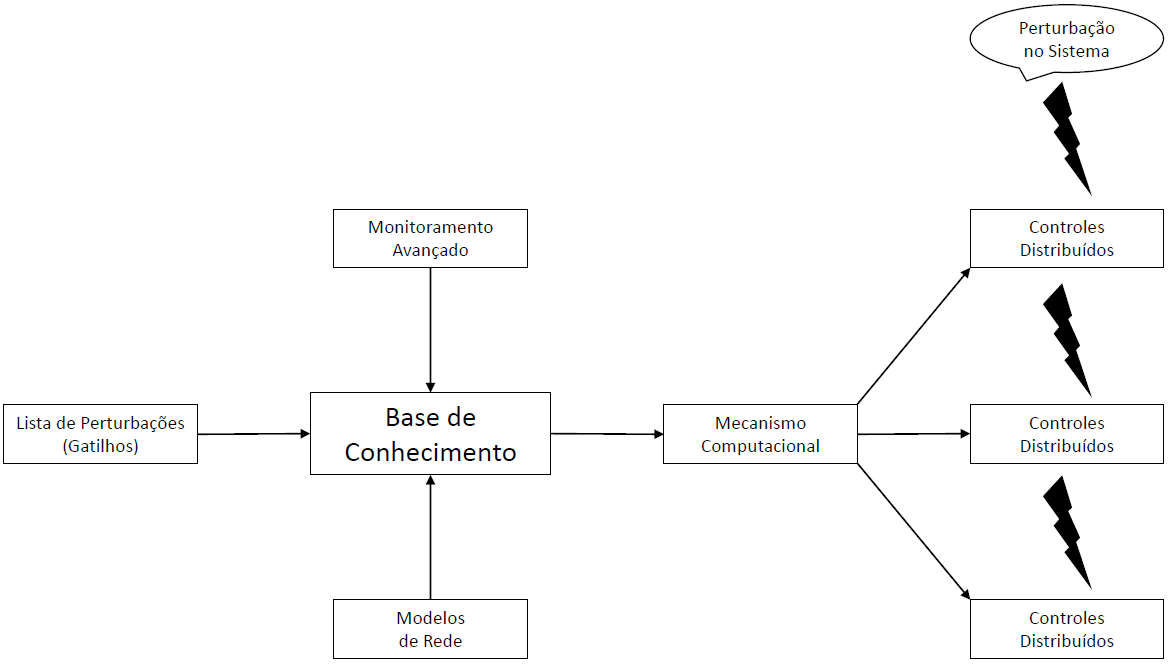
\includegraphics[width=\linewidth]{figuras/ilsdiag}
	\caption[\textbf{ILS}]{\textbf{ILS} [Fonte: \citeauthor{1518342}, adaptado]}
	\label{fig:ilsdiag}
\end{figure}

\subsection{\textbf{ILS} \--- Sistemas Inteligentes} \label{ssec:ils}

H{\'a} diversos tipos de modelos \textbf{ILS}; alguns determin{\'\i}sticos, que utilizam ranqueamento \cite{wang2014, verayiah2015}; outros baseados em algoritmos de minimiza{\c c}{\~a}o de custos (ou maximiza{\c c}{\~a}o de benef{\'\i}cios), como algoritmos gen{\'e}ticos; h{\'a} os que se baseiam em L{\'o}gica \textit{Fuzzy}; e, ainda, as \textbf{ANN} (\textit{Artificial Neural Network}), que s{\~a}o as Redes Neurais Artificiais \cite{yan2017, santos2014}. O objetivo destes modelos \cite{7046661} {\'e} agregar a experi{\^e}ncia do engenheiro que projeta o sistema, de forma a otimizar a decis{\~a}o tomada. Assim, o que a maioria dos modelos \textbf{ILS} t{\^e}m em comum {\'e} a utiliza{\c c}{\~a}o de {\'\i}ndices de ranqueamento, pesos, ou, em ingl{\^e}s, \textit{weights}. Esses {\'\i}ndices s{\~a}o definidos pelo projetista do sistema em lugar da tabela est{\'a}tica, geralmente dentro de uma escala de valores definida, sendo, por exemplo, n{\'u}meros inteiros entre $0$ e $10$.

Em \cite{B574}, encontra-se um modelo determin{\'\i}stico que utiliza fatores combinados e classifica{\c c}{\~a}o direta. Assim, em vez de definir pesos atribu{\'\i}dos {\`a}s cargas definindo a import{\^a}ncia geral, eram atribu{\'\i}dos pesos por cen{\'a}rios e esses ficavam dispon{\'\i}veis ao operador para serem escolhidos durante a opera{\c c}{\~a}o, gerando a flexibilidade de escolher a prioridade por sistema dentro da planta industrial. Em uma aplica{\c c}{\~a}o mais generalizada, poderia ser definido em termos de {\'a}rea f{\'\i}sica de distrubui{\c c}{\~a}o em vez de sistema.  Estes {\'\i}ndices s{\~a}o combinados a outros m{\'e}todos dentro do algoritmo adotado para gerar uma classifica{\c c}{\~a}o final, que pode variar de acordo com o cen{\'a}rio ou, ainda, a subesta{\c c}{\~a}o onde o \textbf{ILS} ser{\'a} disparado. Esta classifica{\c c}{\~a}o era aplicada a um modelo matem{\'a}tico que combinava outros fatores, sendo o principal, a pot{\^e}ncia el{\'e}trica medida em tempo real. Entretanto, as limita{\c c}{\~o}es que ele possui e por conta de avan{\c c}os nos recursos computacionais dispon{\'\i}veis, houve a reformula{\c c}{\~a}o completa desta filosofia.

\section{Implementa{\c c}{\~o}es} \label{sec:casos}

O Governo brasileiro, atrav{\'e}s da \citeauthoronline{aneel2015}, estabeleceu o \textbf{ERAC} (Esquema Regional de Al{\'\i}vio de Carga por Sub-Frequ{\^e}ncia), definindo como:

\begin{quote}
	``Sistema de prote{\c c}{\~a}o que, por meio do desligamento autom{\'a}tico e escalonado de blocos de carga, utilizando rel{\'e}s de frequ{\^e}ncia, minimiza os efeitos de subfrequ{\^e}ncia decorrentes de perda de grandes blocos de gera{\c c}{\~a}o.'' \cite[p.~156]{aneel2015}
\end{quote}

A partir da defini{\c c}{\~a}o do \textbf{ERAC}, coube ao \citeauthor{iogcbr02} sua regulamenta{\c c}{\~a}o e implementa{\c c}{\~a}o. Este define os ajustes do \textbf{ERAC} por regi{\~a}o ou {\'a}rea el{\'e}trica, fornecendo tabelas com valores para cada uma por faixa de frequ{\^e}ncia, incluindo bancos de capacitores em subesta{\c c}{\~o}es. H{\'a} duas formas definidas para atua{\c c}{\~a}o do \textbf{ERAC}: valor absoluto e queda acentuada na frequ{\^e}ncia. O \citeauthoronline{iogcbr02} \cite[item 2.1.3]{iogcbr02} define ainda o tempo de atua{\c c}{\~a}o para disparo do est{\'a}gio, sendo cinco est{\'a}gios para cada tabela de atua{\c c}{\~a}o. Este tempo est{\'a} definido como nove ciclos el{\'e}tricos ($150ms$), sendo tr{\^e}s para detec{\c c}{\~a}o e seis para abertura dos disjuntores. Assim, dependendo da velocidade da queda de frequ{\^e}ncia, do valor que esta atinja e da {\'a}rea de opera{\c c}{\~a}o onde ocorra, uma etapa de rejei{\c c}{\~a}o de cargas {\'e} disparada para o percentual de carga correspondente nas tabelas encontradas em \cite{iogcbr02}.

Apesar do modelo consolidado no Brasil, diversos estudos ainda est{\~a}o em curso buscando novas metodologias. Por exemplo, \citeauthor{li2006} estudaram a influ{\^e}ncia das caracter{\'\i}sticas das cargas, como motores s{\'\i}ncronos ou imped{\^a}ncia fixa, e apresentaram seus efeitos sobre a frequ{\^e}ncia em cen{\'a}rios de sub-tens{\~a}o, utilizando simula{\c c}{\~a}o para realizar um estudo de caso da rede el{\'e}trica da cidade de Beijing, no norte da China.

J{\'a} \citeauthor{kucuk2018} modela um sistema industrial, realizando estudo de caso considerando uma refinaria de petr{\'o}leo. \citeauthoronline{kucuk2018} estuda os efeitos do aumento na demanda dos geradores visando aliviar a carga para prevenir uma poss{\'\i}vel sobrecarga. Este caso {\'e} interessante, pois as refinarias t{\^e}m muito em comum com plataformas de produ{\c c}{\~a}o, embora a grande diferen{\c c}a seja a conex{\~a}o ao sistema de transmiss{\~a}o que as refinarias geralmente disp{\~o}em. Entretanto, as caracter{\'\i}sticas das plantas industriais, em oposi{\c c}{\~a}o {\`a}s instala{\c c}{\~o}es comerciais ou sistemas urbanos de distribui{\c c}{\~a}o, t{\^e}m como cargas majorit{\'a}rias motores de grande porte. Assim, \citeauthor{ye2015zhe} comparam o efeito de descartar motores em compara{\c c}{\~a}o {\`a} mesma quantidade de outros tipos de carga, demonstrando que descartar motores primeiro oferece uma vantagem maior na recupera{\c c}{\~a}o, tanto da tens{\~a}o quanto da frequ{\^e}ncia da rede.

Al{\'e}m dos efeitos el{\'e}tricos, h{\'a} ainda um efeito econ{\^o}mico no desligamento. Neste trabalho, como o foco est{\'a} nos sistemas isolados, a quest{\~a}o econ{\^o}mica resume-se ao custo de parada dos equipamentos e da sua produ{\c c}{\~a}o relativa. Entretanto, em sistemas de transmiss{\~a}o, distribui{\c c}{\~a}o e comercializa{\c c}{\~a}o de energia, h{\'a} o valor da pr{\'o}pria energia n{\~a}o entregue. Assim, \citeauthor{tikdari2015} realizaram um estudo onde contabilizaram, junto a outras restri{\c c}{\~o}es, o custo marginal da energia. Tal linha de racioc{\'\i}nio tamb{\'e}m foi seguida por \citeauthor{paul2017}.

Outro aspecto a ser considerado nos sistemas \textbf{ILS} {\'e} a velocidade em que as solu{\c c}{\~o}es s{\~a}o computadas. Em outras palavras, h{\'a} a necessidade de adequar os algoritmos e limita{\c c}{\~o}es de hardware existentes {\`a} velocidade requerida para a atua{\c c}{\~a}o. Ali{\'a}s, este tem sido o real motivo para as redes de grande porte utilizarem os rel{\'e}s de atua{\c c}{\~a}o com tabelas est{\'a}ticas. Os modelos puramente classificadores, como o que foi proposto em \cite{B574}, trazem consigo a vantagem de ter seus c{\'a}lculos computados offline, de forma que, na necessidade de atua{\c c}{\~a}o, os resultados j{\'a} estejam dispon{\'\i}veis. Face a esta limita{\c c}{\~a}o, \citeauthor{wester2014} propuseram um esquema de atua{\c c}{\~a}o r{\'a}pida baseado em medi{\c c}{\~o}es de campo, avaliando o balan{\c c}o entre gera{\c c}{\~a}o e carga em tempo real.

\chapter{Metodologia} \label{cap:metod}

Visando determinar um crit{\'e}rio para sele{\c c}{\~a}o das cargas a serem descartadas que atenda aos requisitos de velocidade (estando dispon{\'\i}vel sempre que houver necessidade de atua{\c c}{\~a}o do rel{\'e}), praticidade (visando otimizar a escolha das cargas para preservar as mais importantes) na forma din{\^a}mica e adaptativa (buscando retirar o menor n{\'u}mero poss{\'\i}vel de cargas, minimizando os impactos sobre a rede), o modelo adotado neste trabalho baseia-se em meta-heur{\'\i}stica, tendo como filosofia a atua{\c c}{\~a}o preditiva.

A atua{\c c}{\~a}o do sistema de rejei{\c c}{\~a}o seguir{\'a} a metodologia \textbf{UFLS}, conforme apresentada por \citeauthor{amelirole}, sendo a mesma adotada no Sistema El{\'e}trico Brasileiro \cite{aneel2015}. Um ajuste em cinco etapas ser{\'a} utilizado, podendo se utilizar menos etapas conforme a implementa{\c c}{\~a}o. Assim, a tabela de rejei{\c c}{\~a}o conter{\'a} cinco blocos de cargas, sendo um para cada etapa, para atua{\c c}{\~a}o em cascata, conforme haja necessidade.

A partir da defini{\c c}{\~a}o precedente, dada a etapa de desligamento, a entrada do algoritmo que efetuar{\'a} a ordena{\c c}{\~a}o de cargas para gerar sua respectiva tabela receber{\'a} como entrada o ajuste de pot{\^e}ncia de cada etapa e as cargas em opera{\c c}{\~a}o com suas respectivas demandas e pesos de opera{\c c}{\~a}o. Como valores de ajuste (\textit{set points}), este contar{\'a} com os crit{\'e}rios de opera{\c c}{\~a}o e seus respectivos pesos globais e individuais, conforme ser{\'a} detalhado mais adiante na Sube{\c c}{\~a}o~\ref{subsec:f3}. Utilizando esta entrada e estes ajustes, um algoritmo de busca meta-heur{\'\i}stica far{\'a} sucessivas permuta{\c c}{\~o}es visando otimizar a tabela. Ap{\'o}s um intervalo de tempo definido, o sistema atualizar{\'a} as leituras de campo, encerrando a busca para os par{\^a}metros atuais e iniciando uma nova a partir dos valores recebidos.

O crit{\'e}rio de otimiza{\c c}{\~a}o {\'e} uma fun{\c c}{\~a}o l{\'o}gica que constitui a proposta deste trabalho, a qual chamaremos de Fun{\c c}{\~a}o Objetivo\footnote{Ou Fun{\c c}{\~a}o de Custo}, estando na Se{\c c}{\~a}o~\ref{sec:obj}.

\section{Meta-Heur{\'\i}stica de Busca} \label{sec:meth}

A busca que ser{\'a} realizada aqui assemelha-se ao problema do Caixeiro Viajante \cite{applegate2006traveling} que consiste em, dada uma lista de cidades e uma matriz com os custos de deslocamento entre elas, encontrar a ordem em que um caixeiro viajante consegue percorrer todas as cidades sem repeti{\c c}{\~a}o, ao menor custo. No problema original, o {\'u}ltimo ponto {\'e} igual ao primeiro, pois o caixeiro retorna ao ponto de origem. J{\'a} no problema das cargas, n{\~a}o h{\'a} nenhuma repeti{\c c}{\~a}o. Portanto, quaisquer m{\'e}todos de busca que possam resolver este problema cl{\'a}ssico podem ser adotados aqui, sendo a escolha influenciada mais pelo tempo de converg{\^e}ncia para um {\'o}timo local do que para uma solu{\c c}{\~a}o exaustiva. Neste trabalho ser{\'a} adotado o m{\'e}todo \textbf{VND} \--- \textit{Variable Neighborhood Descent} \cite{hansen2001449,hansen2019}, por oferecer r{\'a}pida converg{\^e}ncia para aplica{\c c}{\~a}o em tempo real, caracterizado pela Equa{\c c}{\~a}o~\ref{eq:VNDobj}, cuja solu{\c c}{\~a}o alcan{\c c}a-se atrav{\'e}s do Algoritmo~\ref{alg:vnd}.

\begin{equation} \label{eq:VNDobj}
    min \left\{ f \left( x \right) | x \in \mathcal{X}, \mathcal{X} \subseteq \mathcal{S} \right\}
\end{equation}

Onde,

\begin{itemize}
    \item[] $x$ {\'e} uma solu{\c c}{\~a}o buscada (avaliada);
    \item[] $f \left( x \right)$ {\'e} a fun{\c c}{\~a}o de custo ou fun{\c c}{\~a}o objetivo;
    \item[] $\mathcal{X}$ {\'e} o espa{\c c}o de busca (solu{\c c}{\~o}es avali{\'a}veis);
    \item[] $\mathcal{S}$ {\'e} o espa{\c c}o total de solu{\c c}{\~o}es poss{\'\i}veis.
\end{itemize}

\begin{algorithm}[!h]
	\caption[\textbf{VND} \--- \textit{Variable Neighborhood Descent}]{\textbf{VND} \--- \textit{Variable Neighborhood Descent} [Fonte: \citeauthor{hansen2019}, Figura~6.1, adaptado]}
	\label{alg:vnd}
	\begin{algorithmic}
		\STATE{In{\'\i}cio}
		\STATE{Seleciona o conjunto de estruturas de vizinhan{\c c}a $\mathcal{N}_{k}$, para $k=1, \dots, k_{max}$, que ser{\'a} utilizado na busca}
		\STATE{Encontra uma solu{\c c}{\~a}o inicial $x$}
		\STATE{Escolhe uma condi{\c c}{\~a}o de parada}
		\WHILE{Condi{\c c}{\~a}o de parada n{\~a}o satisfeita}
			\STATE{$k \leftarrow 1$}
			\WHILE{$k \ne k_{max}$}
				\STATE{Gera um ponto $x'$ aleatoriamente a partir da $k-esima$ vizinhan{\c c}a de $x$ ($x' \in \mathcal{N}_{k}\left( x \right)$)}
				\IF{$f \left( x' \right) < f \left( x \right)$}
				    \STATE{$x \leftarrow x'$}
				    \STATE{$k \leftarrow 1$}
				\ELSE
				    \STATE{$k \leftarrow k + 1$}
				\ENDIF
			\ENDWHILE
		\ENDWHILE
	\end{algorithmic}
\end{algorithm}

Para utilizar o \textbf{VND}, portanto, deve-se escolher estruturas de vizinhan{\c c}a de ordens sucessivas e alternar la{\c c}os de busca com a menor vizinhan{\c c}a no la{\c c}o mais interno. Assim, o primeiro passo {\'e} definir as estruturas de vizinhan{\c c}a.

A vizinhan{\c c}a de primeira ordem, $\mathcal{N}_{1}$, ser{\'a} definida como a troca entre elementos com {\'\i}ndices $i$ e $j$ limitados a $n$, ou seja, uma altera{\c c}{\~a}o na ordem de duas cargas destinadas ao desligamento. Isso permite ao termo da fun{\c c}{\~a}o de custo que ir{\'a} tratar da prioridade na ordena{\c c}{\~a}o encontrar uma ordem mais adequada para um conjunto de $n$ cargas, pois se a frequ{\^e}ncia equilibrar-se antes da {\'u}ltima carga no conjunto ser descartada, conv{\'e}m que a carga preservada seja a mais importante. Trata-se de uma otimiza{\c c}{\~a}o do conjunto j{\'a} encontrado. O melhor resultado obtido ser{\'a} considerado um m{\'\i}nimo local.

A vizinhan{\c c}a de segunda ordem, $\mathcal{N}_{2}$, ser{\'a} definida como a troca entre uma carga de {\'\i}ndice $i$ limitado a $n$ e {\'\i}ndice $j$ superior a $n$. Na pr{\'a}tica, trata-se de uma troca entre um elemento que seria descartado por outro que se manteria. Na pr{\'a}tica, isso significa migrar de uma vizinhan{\c c}a para outra em busca de um novo m{\'\i}nimo local.

Uma vizinhan{\c c}a de terceira ordem, $\mathcal{N}_{3}$, seria a troca entre dois elementos de {\'\i}ndices maiores que $n$. Entretanto, trocar a ordem de duas cargas fora do conjunto a ser desligado n{\~a}o faz sentido e, portanto, n{\~a}o ser{\'a} definido.

Uma alternativa ao \textbf{VND} {\'e} o \textit{Iterated Local Search} \cite{lourencco2019}. A implementa{\c c}{\~a}o deste m{\'e}todo requer uma perturba{\c c}{\~a}o quando a solu{\c c}{\~a}o n{\~a}o apresenta mais melhoria com a varia{\c c}{\~a}o das vizinhan{\c c}as locais. O objetivo desta perturba{\c c}{\~a}o {\'e} fugir de valores m{\'\i}nimos locais, procurando uma regi{\~a}o mais distante, fora das estruturas de vizinhan{\c c}a, que pode conter um m{\'\i}nimo local mais vantajoso. Esta perturba{\c c}{\~a}o ser{\'a} definida como uma invers{\~a}o total na ordem das cargas na melhor solu{\c c}{\~a}o encontrada\footnote{Embora esta perturba{\c c}{\~a}o seja parte do algoritmo \textbf{ILS}, ela n{\~a}o foi implementada neste trabalho, sendo utilizado, portanto, o \textbf{VND} apenas. Ela est{\'a} apresentada aqui como uma implementa{\c c}{\~a}o alternativa para melhoria em trabalhos futuros.}.

Sempre que uma solu{\c c}{\~a}o resultar em um custo inferior ao melhor custo obtido, este ser{\'a} atualizado e a busca ser{\'a} reiniciada utilizando este novo resultado como solu{\c c}{\~a}o inicial, ou seja, a busca retorna ao espa{\c c}o da vizinhan{\c c}a $\mathcal{N}_{1}$, conforme o Algoritmo~\ref{alg:vnd}.

Como existe uma in{\'e}rcia no sistema em opera{\c c}{\~a}o normal, a cada nova leitura, no caso de n{\~a}o haver mudan{\c c}a topol{\'o}gica ou entrada e sa{\'\i}da de elementos da rede, a solu{\c c}{\~a}o da busca anterior ser{\'a} utilizada como ponto de partida (solu{\c c}{\~a}o inicial) para a busca seguinte. Entretanto, cada vez que uma carga entra ou sai de opera{\c c}{\~a}o, esta mudan{\c c}a altera a topologia da rede. Assim, havendo mudan{\c c}a na topologia, o vetor de solu{\c c}{\~o}oes que cont{\'e}m as cargas ativas, constituindo o espa{\c c}o de busca, altera seu comprimento, fazendo com que o Algoritmo~\ref{alg:vnd} necessite ser reiniciado. Esta caracter{\'\i}stica aparece nos resultados, j{\'a} que, em cada novo in{\'\i}cio, o resultado converge de forma mais r{\'a}pida, com uma tend{\^e}ncia a se estabilizar em torno de uma solu{\c c}{\~a}o. A Se{\c c}{\~a}o~\ref{sec:anares} apresentar{\'a} em detalhes como isso ocorre na pr{\'a}tica.

A forma final do esquema adotado neste trabalho est{\'a} apresentada no Algoritmo~\ref{alg:lsgeral}, que apresenta as etapas gerais da metodologia proposta, e a busca com a meta-heur{\'\i}stica adotada, no Algoritmo~\ref{alg:lsbusca}.



\begin{algorithm}[h]
	\caption{Algoritmo de Busca para Rejei{\c c}{\~a}o de Cargas - Vis{\~a}o Geral}
	\label{alg:lsgeral}
	\begin{algorithmic}
		\STATE{In{\'\i}cio}
		\STATE{Ordena as cargas em opera{\c c}{\~a}o utilizando os fatores de opera{\c c}{\~a}o como solu{\c c}{\~a}o inicial (classifica{\c c}{\~a}o direta)}
		\WHILE{Sistema Operando}
			\STATE{Recebe leitura do campo com o estado do sistema}
			\WHILE{N{\~a}o h{\'a} nova leitura dispon{\'\i}vel}
				\STATE{Aciona algoritmo de busca}
			\ENDWHILE
		\ENDWHILE
	\end{algorithmic}
\end{algorithm}

\begin{algorithm}[h]
	\caption{Algoritmo de Busca para Rejei{\c c}{\~a}o de Cargas - Meta-Heur{\'\i}stica}
	\label{alg:lsbusca}
	\begin{algorithmic}
		\STATE{In{\'\i}cio}
		\STATE{Recebe estado do sistema}
		\STATE{Salva a solu{\c c}{\~a}o atual como melhor}
		\STATE{Calcula e armazena custo da solu{\c c}{\~a}o atual como melhor}
		\WHILE{Estado se mant{\'e}m}
			\WHILE{Melhor solu{\c c}{\~a}o se altera}
				\FOR{$i$ dentro do n{\'u}mero de cargas ativas}
					\FOR{j dentro do n{\'u}mero de cargas ativas e $j>i$}
						\STATE{$S$ $\leftarrow$ Troca a ordem das cargas $i$ e $j$}
						\IF{Custo de $S$ menor que melhor custo}
							\STATE{Atualiza a melhor solu{\c c}{\~a}o}
							\STATE{Atualiza melhor custo}
							\STATE{Atualiza os rel{\'e}s do sistema de atua{\c c}{\~a}o}
						\ENDIF
					\ENDFOR
				\ENDFOR
			\ENDWHILE
		\ENDWHILE
	\end{algorithmic}
\end{algorithm}

\section{Fun{\c c}{\~a}o Objetivo} \label{sec:obj}

Como mencionado anteriormente, esta fun{\c c}{\~a}o representa efetivamente a contribui{\c c}{\~a}o deste trabalho no sentido de propor uma solu{\c c}{\~a}o para o problema de Rejei{\c c}{\~a}o de Cargas. Diversos trabalhos, conforme indicado no Cap{\'\i}tulo~\ref{cap:revbib}, utilizam sistema \textbf{ILS}, muitos dos quais se baseiam em crit{\'e}rios de busca ou ordena{\c c}{\~a}o. O que os diferencia {\'e}, justamente, o crit{\'e}rio utilizado nesta busca. Assim, a Equa{\c c}{\~a}o~\ref{eq:objsimp} ser{\'a} o crit{\'e}rio adotado aqui.

\begin{equation} \label{eq:objsimp}
	\mathcal{F}\left( x, P \right) = \sum_{i=1}^{4}{C_{i} \times f_{i} \left( x, P \right)}
\end{equation}

Onde,

\begin{itemize}
	\item[] $ x $ {\'e} uma solu{\c c}{\~a}o que consiste em uma lista de valores contendo os {\'\i}ndices das cargas do sistema em uma ordem particular;
	\item[] $ P $ {\'e} a pot{\^e}ncia para descartar no bloco;
	\item[] $ f_{1}\left(x, P \right) $ {\'e} a penalidade por diferen{\c c}a de pot{\^e}ncia retirada;
	\item[] $ f_{2}\left(x, P \right) $ {\'e} a penalidade por n{\'u}mero de cargas retiradas;
	\item[] $ f_{3}\left(x, P \right) $ {\'e} a aplica{\c c}{\~a}o dos crit{\'e}rios de import{\^a}ncia para a opera{\c c}{\~a}o;
	\item[] $ f_{4}\left(x, P \right) $ {\'e} o efeito de ordena{\c c}{\~a}o das cargas retiradas;
	\item[] $ C_{i} $ {\'e} o fator de pondera{\c c}{\~a}o de $ f_{i}\left(x, P \right) $ no somat{\'o}rio.
\end{itemize}

As cinco etapas de desligamento configuradas atuam sucessivamente, mas n{\~a}o necessariamente at{\'e} a {\'u}ltima. Assim, se, por exemplo, a primeira etapa contemplar $10\%$ da carga, e a segunda, $15\%$, ao atuar o primeiro bloco, se a frequ{\^e}ncia come{\c c}ar a recuperar-se, o segundo bloco n{\~a}o chegar{\'a} a atuar, caso contr{\'a}rio, ser{\'a} descartado um montante de $15\%$ aplicado sobre os $90\%$ que restaram na primeira etapa ou seja, $13,5\%$ do montante inicial. Embora cada etapa atue de forma independente, cada bloco depende da defini{\c c}{\~a}o do bloco anterior, j{\'a} que as cargas que comp{\~o}em um bloco n{\~a}o podem ser contempladas no bloco seguinte. Essa depend{\^e}ncia pode ser um problema, pois cada etapa precisa ser definida para come{\c c}ar a busca seguinte. Para contornar esta depend{\^e}ncia, ser{\'a} utilizado um artif{\'\i}cio l{\'o}gico. Dada uma classifica{\c c}{\~a}o de cargas, as primeiras ser{\~a}o alocadas para o primeiro bloco at{\'e} que se tenha os $15\%$ ajustados, as seguintes ser{\~a}o alocadas para o segundo bloco at{\'e} atingir o montante de $13,5\%$ calculado para o ajuste de $15\%$, e assim sucessivamente at{\'e} o quinto bloco. Para equilibrar a classifica{\c c}{\~a}o dos blocos e evitar que o {\'u}ltimo bloco que tem menor probabilidade de atua{\c c}{\~a}o seja avaliado com o mesmo peso do primeiro que dever{\'a} necessariamente atuar, o custo total ser{\'a} uma soma ponderada do custo dos blocos, com fator unit{\'a}rio para o primeiro bloco e descr{\'e}scimo de $0,2$ para cada bloco posterior, conforme consta na Equa{\c c}{\~a}o~\ref{eq:pond}.

\begin{equation} \label{eq:pond}
	f\left( x \right) = \sum_{j=1}^{5}{\sum_{i=1}^{4}{\left(1,2-0,2\times j\right) \times C_{i} \times f_{i} \left( x, P_{j} \right)}}
\end{equation}

\subsection{Propaga{\c c}{\~a}o de Efeitos} \label{subsec:f0}

A fun{\c c}{\~a}o de custo retorna, virtualmente, dois valores, pois uma informa{\c c}{\~a}o obtida na Equa{\c c}{\~a}o~\ref{eq:f0} deve ser levada adiante junto com o custo da solu{\c c}{\~a}o: o valor de $n$ que apresenta o menor custo, ou seja, a quantidade de cargas descartada numa solu{\c c}{\~a}o particular. Esta considera{\c c}{\~a}o torna-se importante, pois causa uma diferen{\c c}a conceitual entre permutar elementos inclusos no conjunto de cargas que ser{\~a}o descartadas e elementos n{\~a}o inclusos. Conforme veremos, isso nos permite definir as vizinhan{\c c}as de forma menos habitual.

\begin{equation} \label{eq:f0}
	f_{0} \left( x, P \right) = \vec{\Pi}
\end{equation}

A fun{\c c}{\~a}o estabelecida na Equa{\c c}{\~a}o~\ref{eq:f0} {\'e} puramente l{\'o}gica e, embora n{\~a}o entre no somat{\'o}rio diretamente, norteia os tr{\^e}s primeiros termos deste. Ela utiliza a matriz de correla{\c c}{\~a}o ou propaga{\c c}{\~a}o. Esta matriz {\'e} bin{\'a}ria, e cada linha corresponde a uma carga indica se o seu desligamento tamb{\'e}m ocasiona o desligamento da carga correspondente {\`a} coluna. Assim, a linha que corresponde a um painel, por exemplo, ter{\'a} todas as colunas correspondentes as suas cargas com valor $True$ (ou seja, $1$). Analogamente, todos os valores na diagonal principal ser{\~a}o verdadeiros.

A sa{\'\i}da desta fun{\c c}{\~a}o ser{\'a} um vetor, tamb{\'e}m bin{\'a}rio (booleano), cujo n{\'u}mero de elementos verdadeiros ser{\'a} o total de cargas desligadas e a posi{\c c}{\~a}o destes corresponde a quais s{\~a}o estas.

Seu c{\'a}lculo consiste unicamente em uma opera{\c c}{\~a}o $ou$ entre os vetores formados pelas $n$ primeiras linhas da matriz de correla{\c c}{\~a}o.

\subsection{Diferen{\c c}a de Pot{\^e}ncia} \label{subsec:f1}

\begin{equation} \label{eq:f1}
	f_{1} \left( x, P \right) = \frac{1}{e^{2}} \frac{\left( P - \left< \vec{P_{x}}, \vec{\Pi} \right> \right)^{2}}{P^{2}}
\end{equation}

Onde,

\begin{itemize}
	\item[] $ P $ {\'e} o valor (escalar) de refer{\^e}ncia para a carga a ser retirada na etapa de desligamento. \'{E} poss{\'\i}vel que seja necess{\'a}rio somar uma unidade no denominador para evitar uma poss{\'\i}vel divis{\~a}o por $0$ caso se trabalhe com inteiros, mas a exclus{\~a}o direta da busca para o caso de uma gera{\c c}{\~a}o nula {\'e} mais eficiente;
	\item[] $ \vec{P_{x}} $ {\'e} o vetor contendo os valores de pot{\^e}ncia das cargas cargas em $x$;
	\item[] $ \vec{\Pi} $ {\'e} o vetor calculado em $f_{0}\left(x, P \right)$;
	\item[] A opera{\c c}{\~a}o $\left< \vec{P_{x}}, \vec{\Pi} \right>$ {\'e} o produto interno entre os vetores.
	\item[] $ e $ {\'e} a toler{\^a}ncia para aplica{\c c}{\~a}o da penalidade. Este valor foi ajustado em $1\%$ nas simula{\c c}{\~o}es.
\end{itemize}

Para realizar este c{\'a}lculo, {\'e} utilizada uma matriz bin{\'a}ria contendo a correla{\c c}{\~a}o entre as cargas. Esta matriz tem a hierarquia referente {\`a} topologia da rede, bem como fatores f{\'\i}sicos adicionais que s{\~a}o monitorados. Esta parte do modelo considerando as correla{\c c}{\~o}es n{\~a}o topol{\'o}gicas n{\~a}o ser{\'a} simulada, apenas conceituada e integra sugest{\~a}o para trabalhos futuros.

\subsection{Abrang{\^e}ncia} \label{subsec:f2}

\begin{equation} \label{eq:f2}
	f_{2} \left( x, P \right) = \frac{k}{N}
\end{equation}

Onde,

\begin{itemize}
	\item[] $ k $ {\'e} o total de unidades de carga descartadas em $x$, considerando os reflexos correspondentes; representa o n{\'u}mero de elementos n{\~a}o nulos em $\vec{\Pi}$, que {\'e} um vetor bin{\'a}rio. Portanto, $k = \left< \vec{\Pi}, \vec{\Pi} \right>$;
	\item[] $ N $ {\'e} o n{\'u}mero de elementos em $x$.
\end{itemize}

\subsection{Crit{\'e}rios de Opera{\c c}{\~a}o} \label{subsec:f3}

\begin{equation} \label{eq:f3}
	f_{3} \left( x, P \right) = diag\left\{ \vec{\Pi} \times \vec{crit}^{T} \right\}
\end{equation}

Onde,

\begin{itemize}
	\item[] $ \vec{crit} = \left( \frac{\sum_{\vec{crit_{0}}}^{\vec{crit_{j}}}{p_{i} \times \vec{crit_{i}}}}{j}\right) $;
	\item[] $ p_{i}$ {\'e} o fator de pondera{\c c}{\~a}o do $i-esimo$ crit{\'e}rio;
	\item[] $ \vec{crit_{i}}$ {\'e} o $i-esimo$ crit{\'e}rio.
\end{itemize}

Este termo representa a inclus{\~a}o dos crit{\'e}rios de prioridade definidos pelo operador do sistema. Assim, uma lista predefinida pelo projetista (que pode ser flexibilizada) disp{\~o}e de uma s{\'e}rie de crit{\'e}rios como, por exemplo, o painel que alimenta uma {\'a}rea f{\'\i}sica espec{\'\i}fica ou um equipamento, colocando a import{\^a}ncia das demais cargas no atendimento {\`a} esta {\'a}rea, ou, ainda, crit{\'e}rios como seguran{\c c}a. A combina{\c c}{\~a}o ponderada desses fatores permite que crit{\'e}rios secund{\'a}rios possam servir como crit{\'e}rio de desempate entre equipamentos equivalentes. Assim, duas bombas com caracter{\'\i}sticas iguais operando em paralelo no mesmo sistema, ao serem classificadas, a que apresentar maior probabilidade de falha mec{\^a}nica pode ser desligada primeiro, aumentando as chances de preserva{\c c}{\~a}o do restante do sistema.

\subsection{Ordena{\c c}{\~a}o} \label{subsec:f4}

\begin{equation} \label{eq:f4}
	f_{4} \left( x, P \right) = \sum_{i=1}^{N}{\left(N-i \right) \times crit_{x_{i}}}
\end{equation}

Onde,

\begin{itemize}
    \item $crit_{x_{i}}$ {\'e} o valor do crit{\'e}rio de opera{\c c}{\~a}o da carga na posi{\c c}{\~a}o $i$ em $x$.
\end{itemize}

A influ{\^e}ncia deste termo deve ser a menor poss{\'\i}vel, servindo apenas como crit{\'e}rio de desempate. Considerando a atua{\c c}{\~a}o por etapas, h{\'a} a possibilidade de n{\~a}o ocorrer a rejei{\c c}{\~a}o de todas as cargas previstas na tabela, de forma que as {\'u}ltimas possam ser preservadas. Portanto, h{\'a} interesse em que cargas menos priorit{\'a}rias sejam descartadas primeiro. Este termo aplica uma pondera{\c c}{\~a}o a mais aos crit{\'e}rios do termo anterior em fun{\c c}{\~a}o da ordem que cada elemento ocupa na tabela, gerando uma penalidade extra. Assim, um peso maior ter seu valor aumentado no in{\'\i}cio da tabela.

\subsection{Fun{\c c}{\~a}o Objetivo Completa} \label{subsec:obj}

\begin{equation} \label{eq:obj}
    f\left( x \right) =
    \sum_{j=1}^{5}\left(1,2-0,2\times j\right) \times
    \left\{
        \begin{matrix}
            C_{1} \times \frac{1}{e^{2}}\frac{\left( P_{j} - \left< \vec{P_{x}}, \vec{\Pi_{j}} \right> \right)^{2}}{P_{j}^{2}} & + \\
            & \\
            C_{2} \times \frac{k_{j}}{N} & + \\
            & \\
            C_{3} \times diag\left\{ \vec{\Pi_{j}} \times \vec{crit}^{T} \right\} & + \\
            & \\
            C_{4} \times \sum_{i=1}^{N}{\left(N-i \right) \times crit_{x_{i}}}
        \end{matrix}
    \right.
\end{equation}

A Equa{\c c}{\~a}o~\ref{eq:obj} {\'e} a forma final da Fun{\c c}{\~a}o Objetivo, considerando os termos definidos acima.

\section{Solu{\c c}{\~a}o Inicial} \label{sec:cldir}

Ao modificar a topologia da rede, atrav{\'e}s da abertura ou fechamento de disjuntores ou chaves seccionadoras, ou seja, ao ligar ou desligar uma carga ou painel, um novo cen{\'a}rio {\'e} gerado. Para fornecer uma solu{\c c}{\~a}o inicial de boa qualidade, utiliza-se a classifica{\c c}{\~a}o direta, utilizando como {\'\i}ndice para tal os crit{\'e}rios de opera{\c c}{\~a}o ($\vec{crit}$) da Equa{\c c}{\~a}o~\ref{eq:f3}. Esta classifica{\c c}{\~a}o servir{\'a} como solu{\c c}{\~a}o inicial para a etapa de busca, devendo, ent{\~a}o, ser otimizada.

\chapter{Simulador Para Rejei{\c c}{\~a}o de Carga} \label{cap:impl}

Para demonstrar  a efetividade do esquema para rejei{\c c}{\~a}o de cargas proposto neste trabalho, foi constru{\'\i}do um simulador digital de sistemas em tempo real, cujas telas de ingresso encontram-se nas Figuras~\ref{fig:sim} a \ref{fig:sim_pumps}. Detalhes do \textit{software} desenvolvido est{\~a}o no Ap{\^e}ndice~\ref{apend:estr}. Trata-se de um simulador que fornece uma \textbf{GUI} (\textit{Graphical User Interface}) que permite ao usu{\'a}rio montar sua pr{\'o}pria rede de testes.

A Figura~\ref{fig:sim_main} apresenta a tela do simulador que cont{\'e}m o painel el{\'e}trico principal, onde os geradores est{\~a}o situados. As Figuras~\ref{fig:sim_panels} e \ref{fig:sim_sub} apresentam telas com cargas que representam pain{\'e}is de distribui{\c c}{\~a}o, enquanto a Figura~\ref{fig:sim_pumps} apresenta cargas que representam alguns motores el{\'e}tricos das bombas industriais. Para ajustar o funcionamento, v{\^e}-se, na Figura~\ref{fig:sim_setpar}, a interface para ajustar os par{\^a}metros da fun{\c c}{\~a}o objetivo, e na Figura~\ref{fig:sim_setls}, as configura{\c c}{\~o}es do sistema de rejei{\c c}{\~a}o autom{\'a}tica de cargas, incluindo tamb{\'e}m o intervalo de atualiza{\c c}{\~a}o das leituras. Esse tempo define o tempo m{\'a}ximo dispon{\'i}vel para cada ciclo de buscas e, durante uma simula{\c c}{\~a}o, ao ser aumentado, permite verificar o desempenho equivalente de um computador com maior capacidade de c{\'a}lculo.

Utilizando a rede configurada pelo usu{\'a}rio, o \textit{software} simula um comportamento din{\^a}mico para a rede, variando aleatoriamente o valor das cargas e distribuindo a demanda pelos geradores ligados ao barramento principal. Na Figura~\ref{fig:sim_main} v{\^e}-se, {\`a} direita, a tabela de desligamento na forma de lista, dividida por etapas de desligamento, onde encontra-se destacado em escala de cores, os elementos que constituem cada etapa. Para tornar essa visualiza{\c c}{\~a}o mais simples, na tela de opera{\c c}{\~a}o, o equipamento que figura em uma das listas tem seu nome destacado com a cor respectiva desta. O sistema tamb{\'e}m permite configurar, atrav{\'e}s da tela apresentada na Figura~\ref{fig:sim_setls} o tempo entre cada ciclo de leituras, sendo este, o tempo de discretiza{\c c}{\~a}o.

Cada rede configurada pelo usu{\'a}rio pode ser armazenada em arquivo para testes posteriores. Assim, para cada arquivo salvo em disco, ao efetuar uma simula{\c c}{\~a}o, o programa gera um \textit{log} contendo os dados b{\'a}sicos para cada cen{\'a}rio gerado e seu respectivo resultado obtido. Este \textit{log} permite uma an{\'a}lise posterior de desempenho, pois com os dados do cen{\'a}rio e de configura{\c c}{\~a}o das constantes de ajuste, um programa sem limite de tempo pode procurar o melhor resultado na ``for{\c c}a bruta'' e compar{\'a}-lo ao resultado obtido em ``tempo real'' pelo algoritmo de busca.

O simulador foi escrito em linguagem de programa{\c c}{\~a}o C++, sendo a interface gr{\'a}fica escrita atrav{\'e}s da \textbf{API} (\textit{Application Programming Interface})\footnote{Interface de programa{\c c}{\~a}o de aplica{\c c}{\~o}es} QtC++\footnote{\url{http://www.qt.io}}. O programa para an{\'a}lise e apresenta{\c c}{\~a}o dos resultados obtidos foi escrito em linguagem Python\footnote{\url{http://www.python.org}}, atrav{\'e}s da interface Jupyter Notebook\footnote{\url{http://www.jupyter.org}}, permitindo mesclar texto, c{\'o}digo, gr{\'a}ficos e leitura/grava{\c c}{\~a}o em arquivo, resultando em uma boa apresenta{\c c}{\~a}o para an{\'a}lise cr{\'\i}tica do simulador. O arquivo contendo a rede constru{\'\i}da pelo usu{\'a}rio foi estruturado em \textbf{JSON} (\textit{JavaScript Object Notation})\footnote{\url{http://www.json.org}} com escrita bin{\'a}ria e extens{\~a}o customizada para o programa, sendo este um formato compacto e de f{\'a}cil manupula{\c c}{\~a}o, ocupando pouco espa{\c c}o em disco. O \textit{log} de opera{\c c}{\~a}o foi definido no formato \textbf{JSON} textual, tornando mais f{\'a}cil a importa{\c c}{\~a}o e tratamento em Python.

Considerando que o escopo deste trabalho n{\~a}o engloba a simula{\c c}{\~a}o detalhada de elementos de din{\^a}mica e controle de sistemas de gera{\c c}{\~a}o, o algoritmo utilizado para fazer o balanceamento de carga\footnote{Tamb{\'e}m conhecido pelo nome em ingl{\^e}s: \textit{Load Sharing}.} foi o mais simples poss{\'\i}vel, fazendo com que os incrementos positivos sejam absorvidos pelo gerador menos carregado percentualmente, enquanto os decr{\'e}scimos, pelos mais carregados, limitando os degraus de acelera{\c c}{\~a}o e desacelera{\c c}{\~a}o {\`a} in{\'e}rcia pr{\'o}pria de cada gerador (constante $H$ definida pela Equa{\c c}{\~a}o~\ref{eq:hinerc}). A tend{\^e}ncia a longo prazo {\'e} o equil{\'\i}brio na carga percentual das m{\'a}quinas. Apesar de simples, esta configura{\c c}{\~a}o {\'e} bastante precisa e veross{\'\i}mil. Todavia, a forma como o simulador foi constru{\'\i}do torna vi{\'a}vel uma melhoria futura, visando implementar algoritmos mais sofisticados para controle de gera{\c c}{\~a}o.

Da mesma forma que o algoritmo de simula{\c c}{\~a}o da gera{\c c}{\~a}o, um algoritmo simplificado simula o comportamento aleat{\'o}rio das cargas el{\'e}tricas. Esta {\'e} a raz{\~a}o dos experimentos realizados aqui serem {\'u}nicos e n{\~a}o serem pass{\'i}veis de reprodu{\c c}{\~a}o exata, j{\'a} que a mesma sequ{\^e}ncia de opera{\c c}{\~o}es, considerando a aleatoriedade de comportamento, leva a resultados distintos. Para definir este comportamento, as cargas foram divididas em duas classes: cargas est{\'a}ticas e cargas din{\^a}micas. As cargas est{\'a}ticas representam, basicamente, pain{\'e}is de distribui{\c c}{\~a}o locais, contendo ilumina{\c c}{\~a}o, tomadas e cargas menores diversas. Estas cargas partem essencialmente desligadas e o algoritmo considera uma varia{\c c}{\~a}o que tende a diminuir quando a carga se aproxima de seu valor nominal, tendendo, assim, a estabilizar a longo prazo. J{\'a} as cargas din{\^a}micas representam os motores de grande porte de unidades industriais. Como caracter{\'\i}stica principal, os motores demandam alta pot{\^e}ncia na partida, assim, o comportamento foi ajustado para estabilizar em torno de $90\%$ da pot{\^e}ncia nominal, e, mesmo apresentando alguma varia{\c c}{\~a}o, tende sempre a retornar a este valor. A velocidade de aumento ou redu{\c c}{\~a}o de carga para motores est{\'a} limitada {\`a} sua in{\'e}rcia mec{\^a}nica associada.

Da mesma forma que a implementa{\c c}{\~a}o do algoritmo de controle de gera{\c c}{\~a}o permite melhoria, este algoritmo de simula{\c c}{\~a}o de carga foi escrito de forma modular, classificado por {\'\i}ndices internos, sendo f{\'a}cil, portanto, a implementa{\c c}{\~a}o de altera{\c c}{\~o}es, tanto da filosofia de simula{\c c}{\~a}o, quanto a insers{\~a}o de novos tipos de carga, com comportamentos distintos. Assim, uma vers{\~a}o mais elaborada pode trabalhar, por exemplo, com o modelo \textbf{ZIP} \cite{guimaraessistemas} para uma representa{\c c}{\~a}o de cargas mais realista, principalmente para estender a cargas n{\~a}o industriais, como sistemas de distribui{\c c}{\~a}o urbana.

\begin{figure}
	\centering
	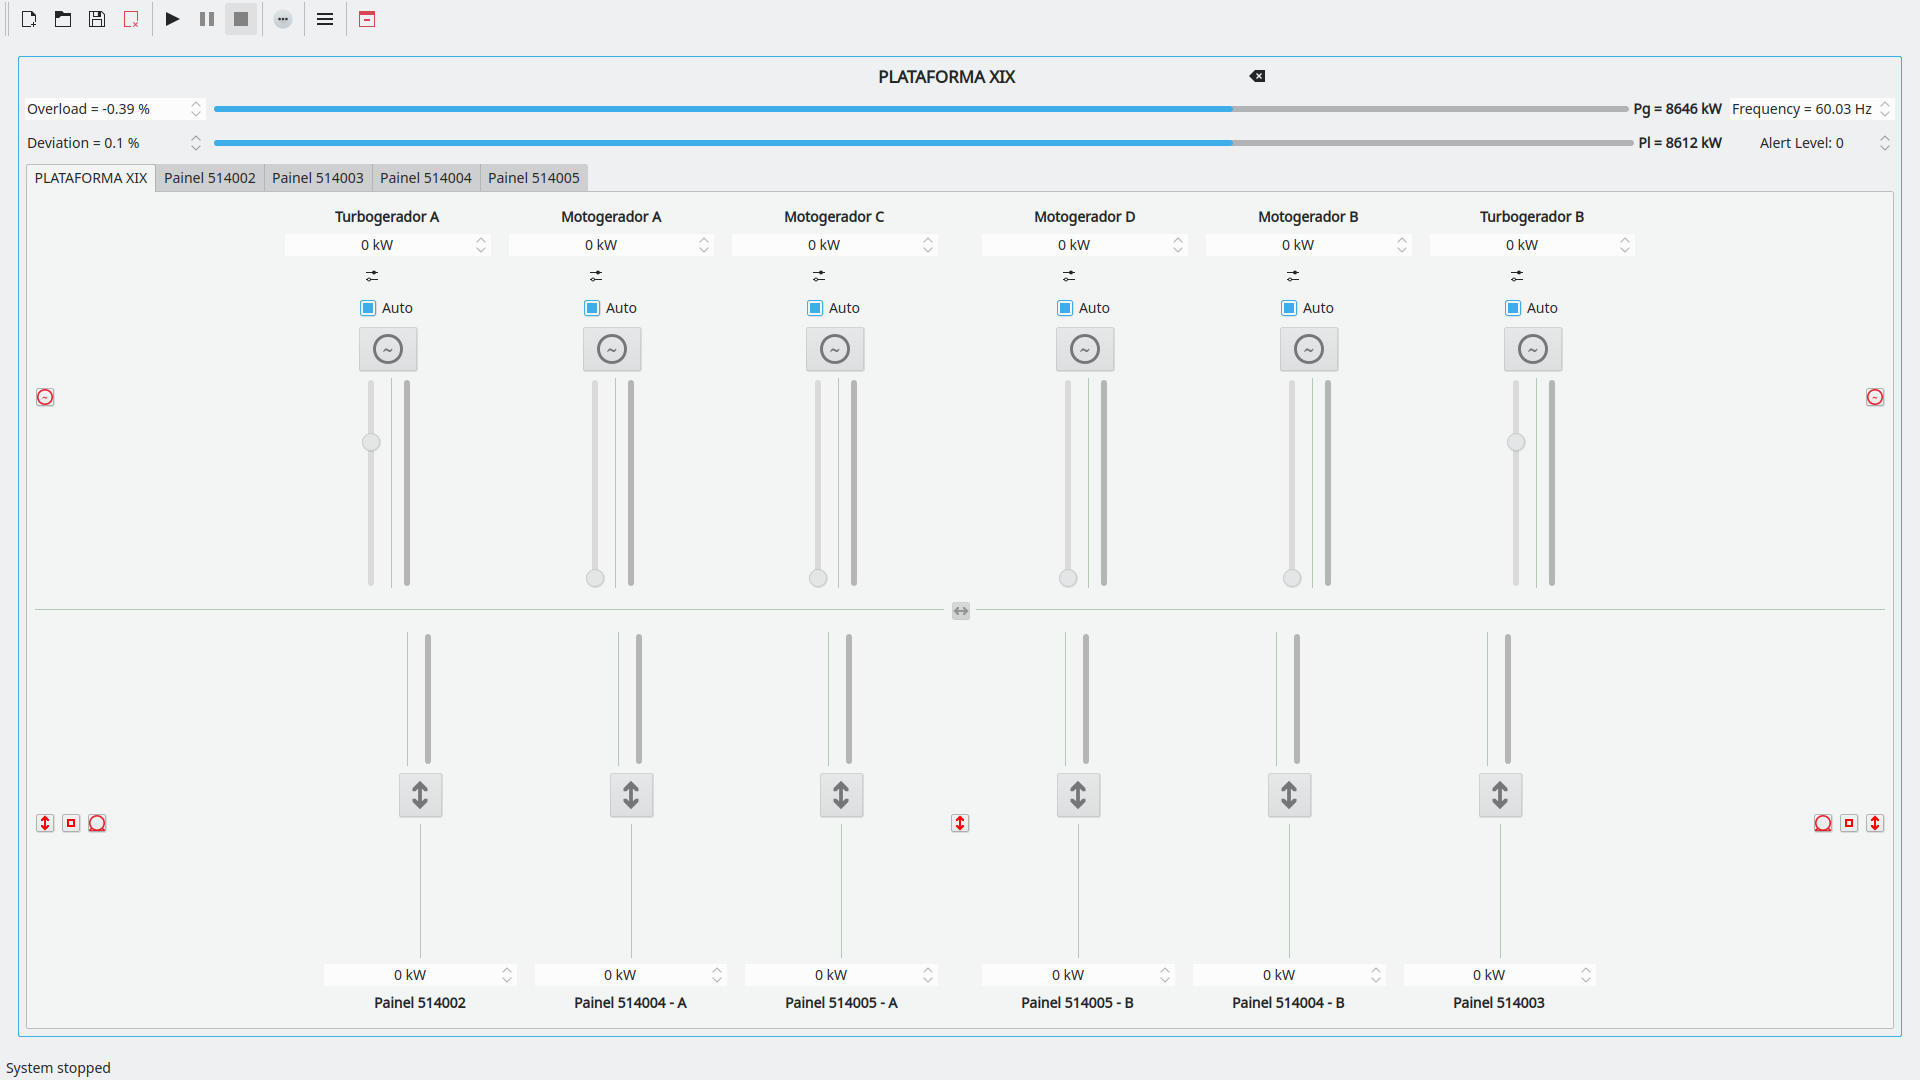
\includegraphics[width=\linewidth]{figuras/simulator}
	\caption[Simulador de Rejei{\c c}{\~a}o de Cargas \---  Tela Inicial]{Simulador de Rejei{\c c}{\~a}o de Cargas \--- Tela Inicial [Fonte: acervo pessoal]}
	\label{fig:sim}
\end{figure}

\begin{figure}
	\centering
	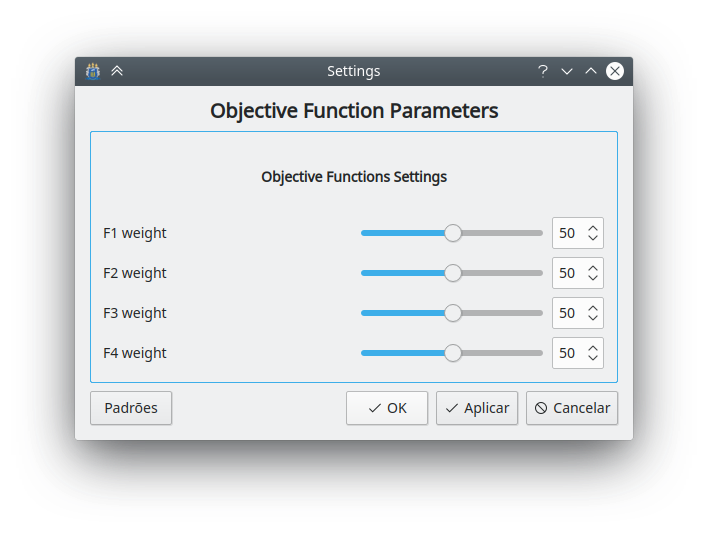
\includegraphics[width=0.8\linewidth]{figuras/parameters}
	\caption[Simulador de Rejei{\c c}{\~a}o de Cargas \--- Par{\^a}metros da Fun{\c c}{\~a}o Objetivo]{Simulador de Rejei{\c c}{\~a}o de Cargas \--- Par{\^a}metros da Fun{\c c}{\~a}o Objetivo [Fonte: acervo pessoal]}
	\label{fig:sim_setpar}
\end{figure}

\begin{figure}
	\centering
	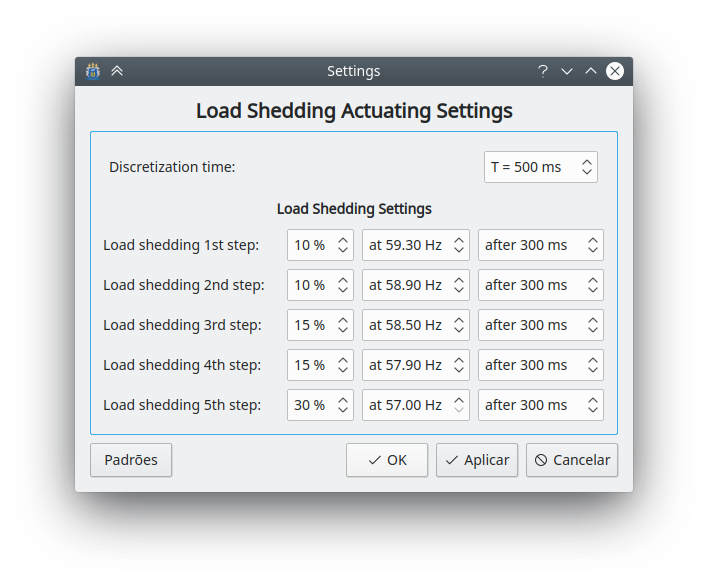
\includegraphics[width=0.8\linewidth]{figuras/settings}
	\caption[Simulador de Rejei{\c c}{\~a}o de Cargas \--- Par{\^a}metros ddo \textbf{UFLS}]{Simulador de Rejei{\c c}{\~a}o de Cargas \--- Par{\^a}metros do \textbf{UFLS} [Fonte: acervo pessoal]}
	\label{fig:sim_setls}
\end{figure}

\begin{figure}
	\centering
	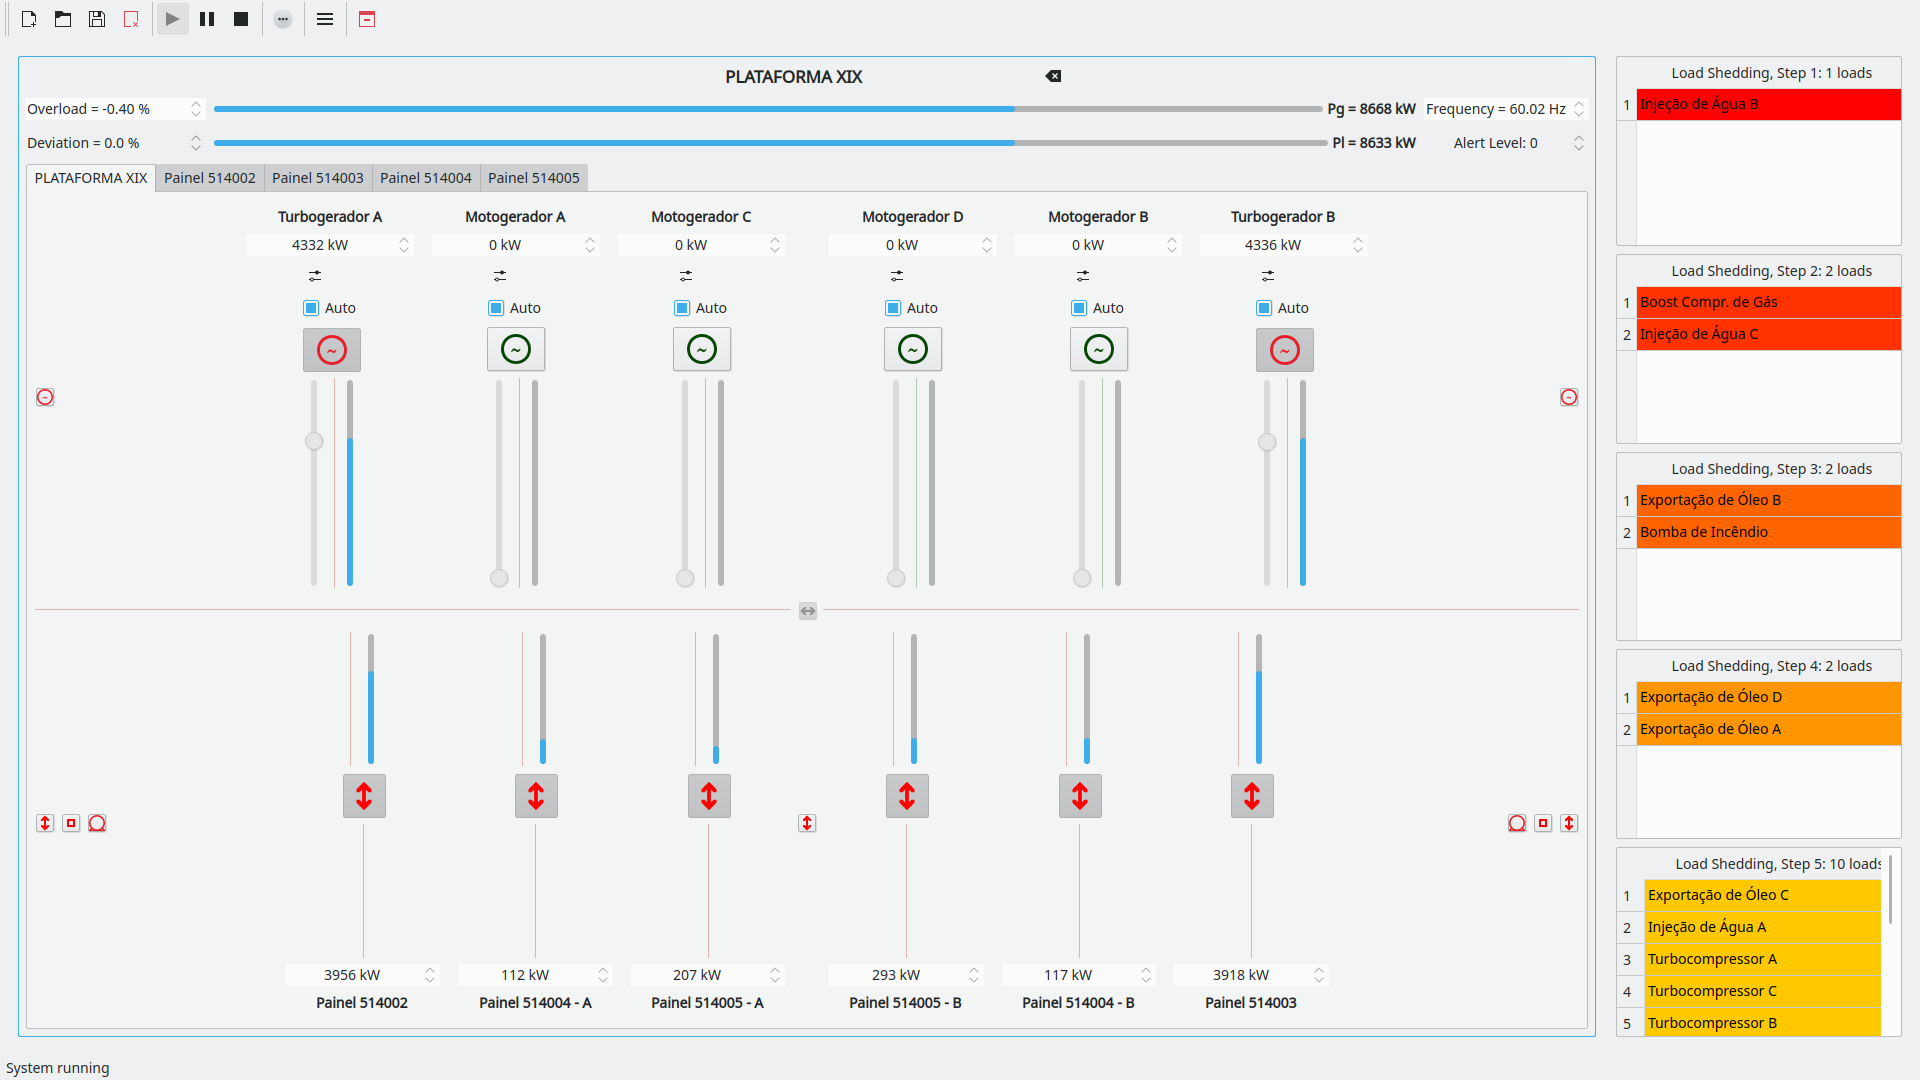
\includegraphics[width=\linewidth]{figuras/simulator_main}
	\caption[Simulador de Rejei{\c c}{\~a}o de Cargas \--- Geradores]{Simulador de Rejei{\c c}{\~a}o de Cargas \--- Geradores [Fonte: acervo pessoal]}
	\label{fig:sim_main}
\end{figure}

\begin{figure}
	\centering
	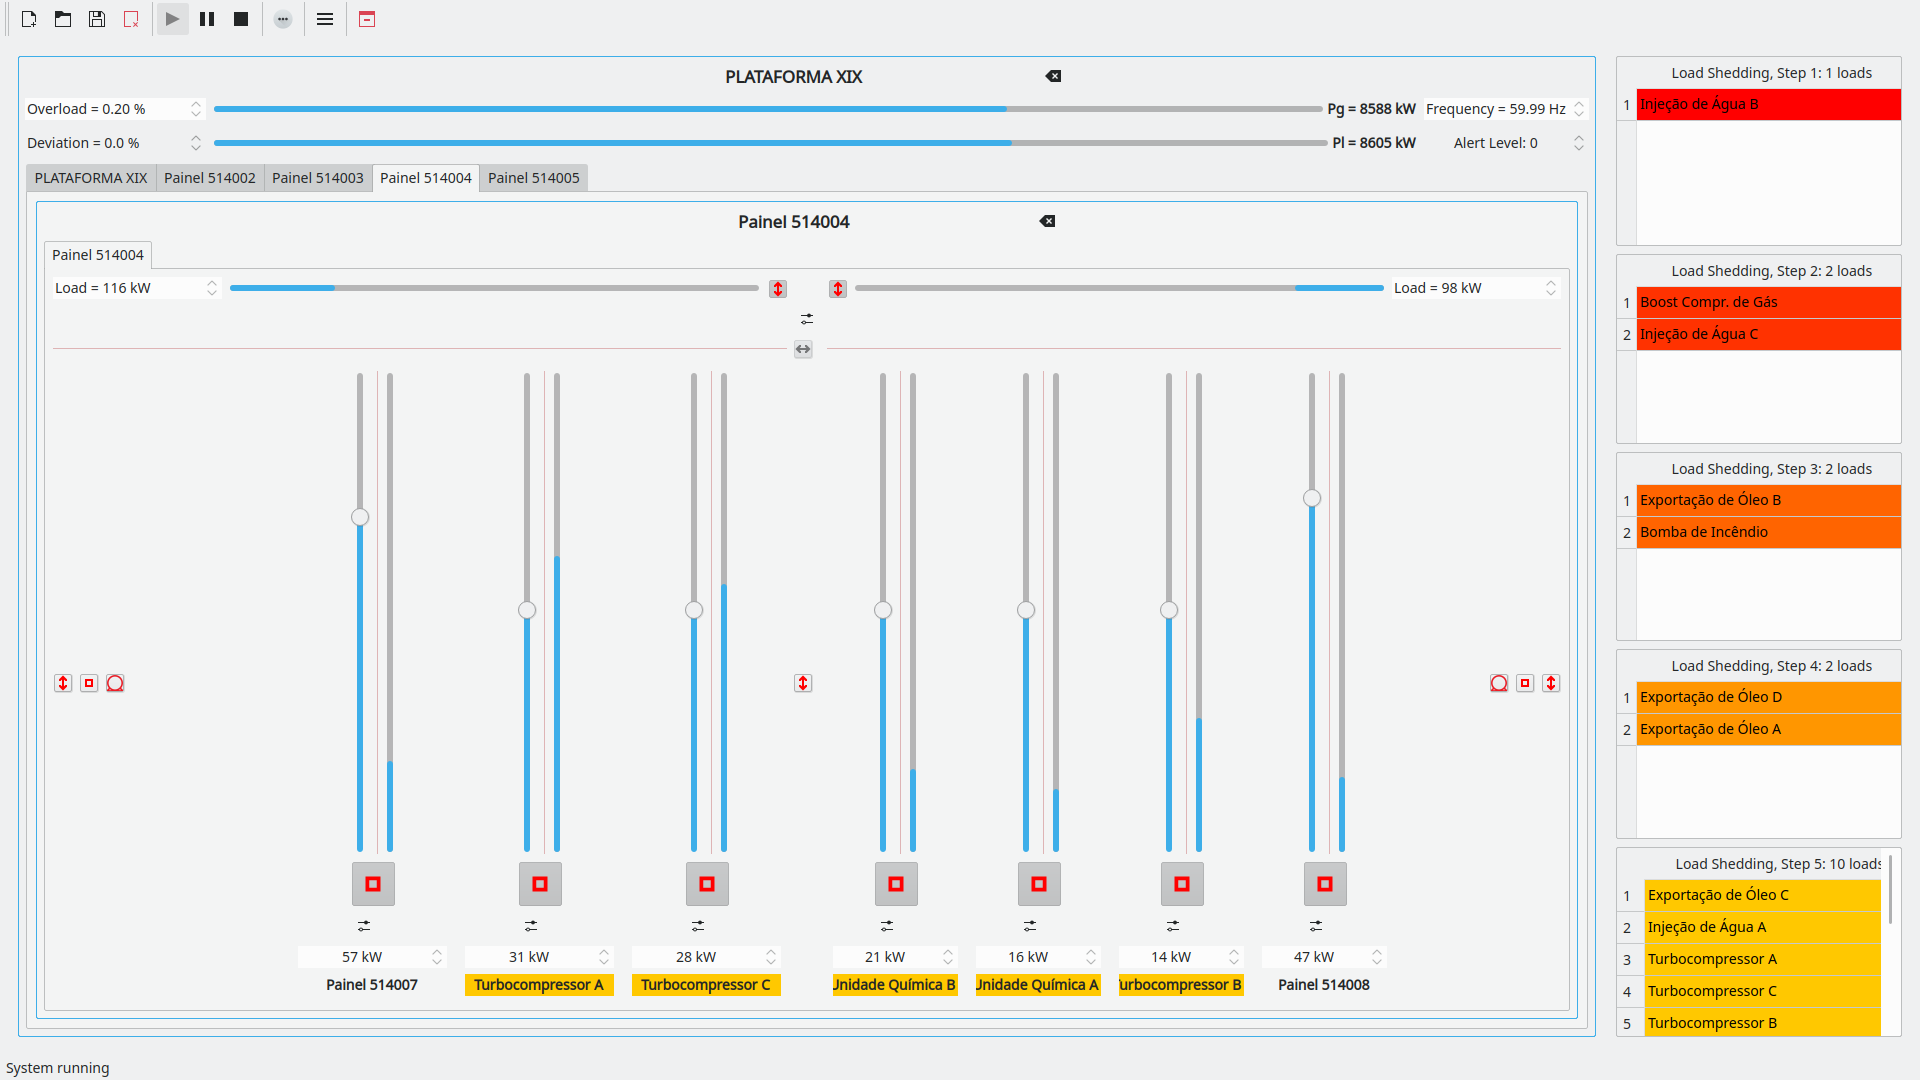
\includegraphics[width=\linewidth]{figuras/simulator_panels}
	\caption[Simulador de Rejei{\c c}{\~a}o de Cargas \--- Pain{\'e}is]{Simulador de Rejei{\c c}{\~a}o de Cargas \--- Pain{\'e}is [Fonte: acervo pessoal]}
	\label{fig:sim_panels}
\end{figure}

\begin{figure}
	\centering
	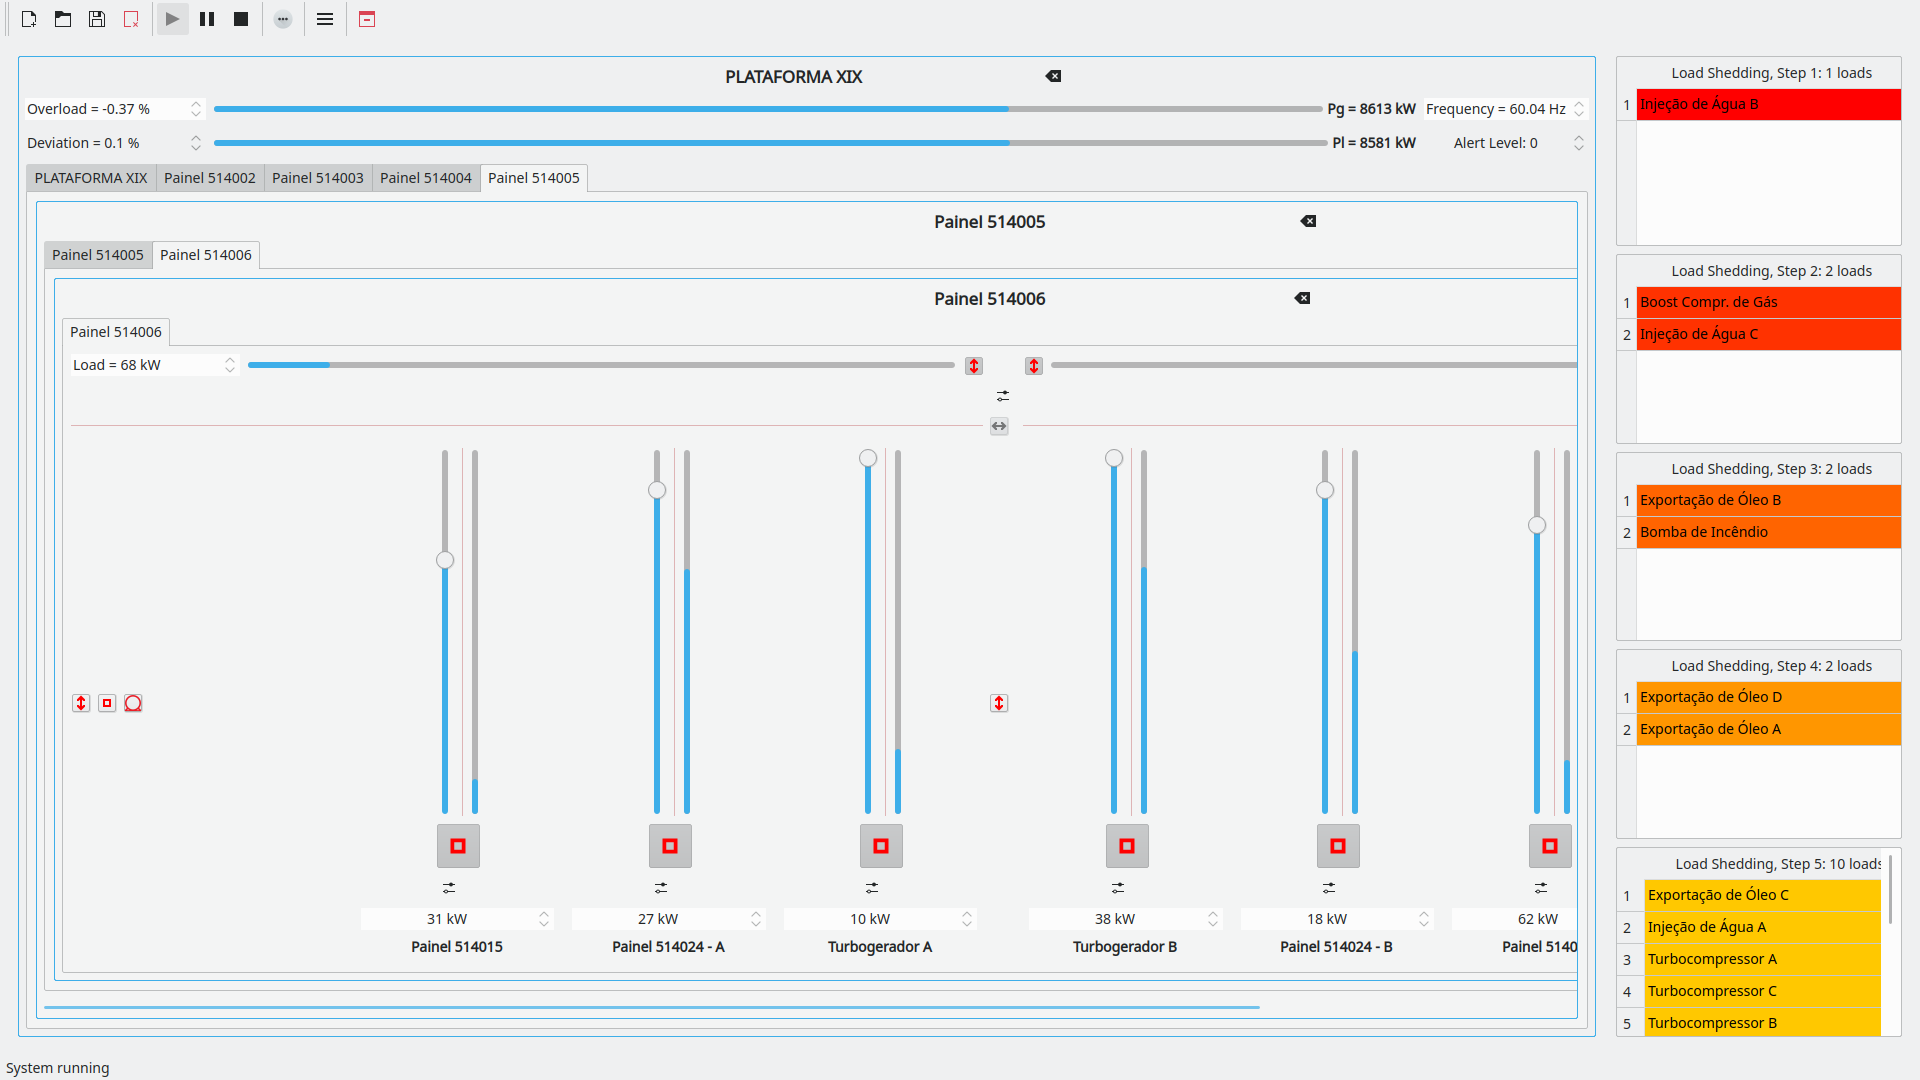
\includegraphics[width=\linewidth]{figuras/simulator_subpanels}
	\caption[Simulador de Rejei{\c c}{\~a}o de Cargas \--- Sub-Pain{\'e}is]{Simulador de Rejei{\c c}{\~a}o de Cargas \--- Sub-Pain{\'e}is [Fonte: acervo pessoal]}
	\label{fig:sim_sub}
\end{figure}

\begin{figure}
	\centering
	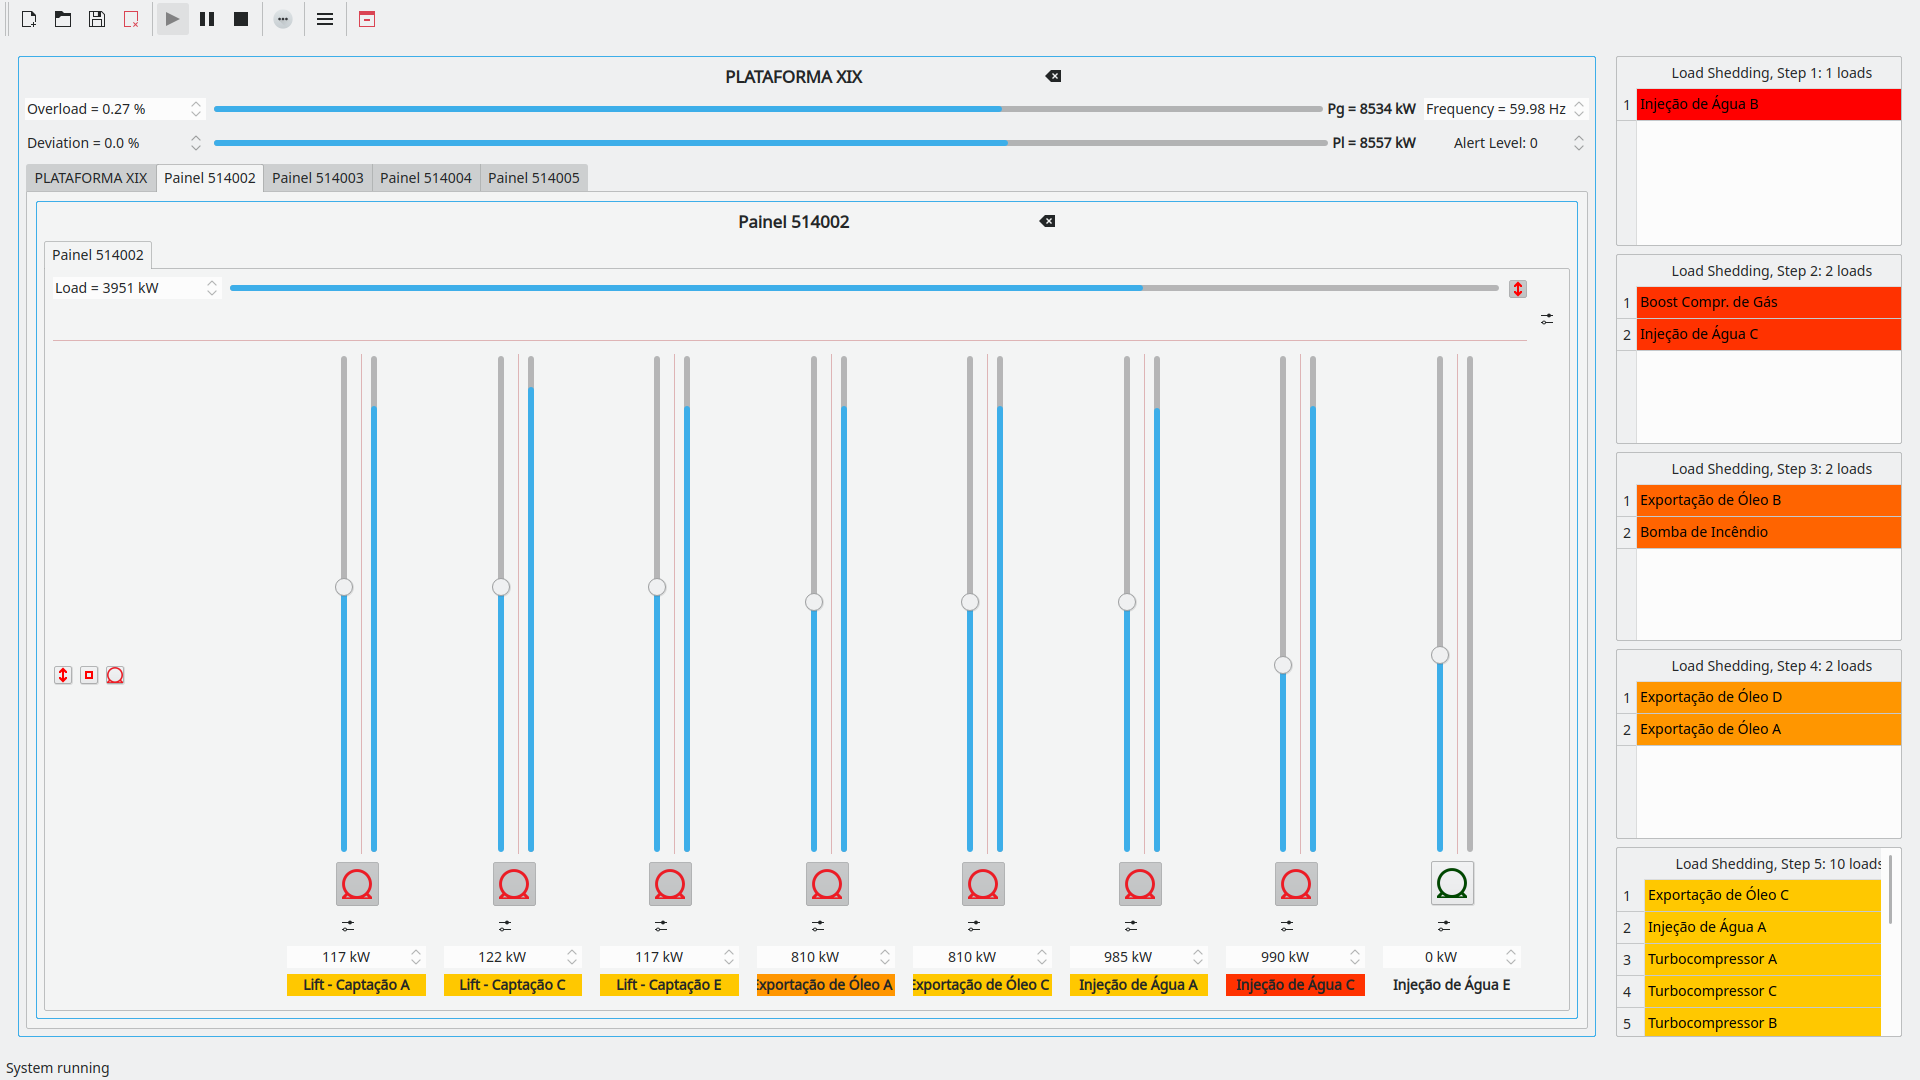
\includegraphics[width=\linewidth]{figuras/simulator_pumps}
	\caption[Simulador de Rejei{\c c}{\~a}o de Cargas \--- Motores de Bombas]{Simulador de Rejei{\c c}{\~a}o de Cargas \--- Motores de Bombas [Fonte: acervo pessoal]}
	\label{fig:sim_pumps}
\end{figure}

\chapter{Resultados} \label{cap:teste}

\section{Planta Utilizada Para Testes} \label{sec:rede}

Para a realiza{\c c}{\~a}o de testes, foi configurada uma rede fict{\'\i}cia, t{\'\i}pica de plataforma de produ{\c c}{\~a}o de petr{\'o}leo em regime \textit{off shore}\footnote{Baseada na experi{\^e}ncia profissional do autor deste trabalho.}. Esta rede cont{\'e}m duas turbinas de gera{\c c}{\~a}o a g{\'a}s natural, com capacidade nominal de $6MW$ de pot{\^e}ncia cada e quatro geradores auxiliares com capacidade nominal de $2MW$ cada, conforme indicado na Tabela~\ref{tab:gen}. Esta configura{\c c}{\~a}o {\'e} comum, pois, em situa{\c c}{\~a}o normal, as plataformas de petr{\'o}leo disp{\~o}em de g{\'a}s oriundo da pr{\'o}pria produ{\c c}{\~a}o para manter as turbinas em opera{\c c}{\~a}o. Em situa{\c c}{\~o}es at{\'\i}picas, como manuten{\c c}{\~a}o ou indisponibilidade de uma turbina, a gera{\c c}{\~a}o faltante {\'e} compensada pela entrada dos geradores auxiliares. Em caso de paradas de produ{\c c}{\~a}o, a plataforma deve se manter utilizando {\'o}leo diesel estocado em tanques, sendo alimentada somente pelos geradores auxiliares\footnote{Em alguns casos, as turbinas a g{\'a}s s{\~a}o bi-combust{\'\i}veis, operando tanto com g{\'a}s quanto diesel.}.

Os geradores s{\~a}o conectados no barramento do painel principal, {\`a}s vezes referido como painel de gera{\c c}{\~a}o ou Subesta{\c c}{\~a}o Principal. Este painel alimenta toda a unidade, atrav{\'e}s de outros pain{\'e}is, conforme Tabela~\ref{tab:loadp1}. As cargas, que consistem em motores, Centros de Controle de Motor \--- CCMs, pain{\'e}is de distribui{\c c}{\~a}o, entre outras, est{\~a}o discriminadas nas Tabelas~\ref{tab:loadp2} a \ref{tab:loadp6}.

\begin{table}[!h]
	\begin{center}
		\caption{Lista de Geradores na Subesta{\c c}{\~a}o Principal}
		\label{tab:gen}
	    \vspace{5pt}
		\begin{tabular}{c c c c}
			\hline
			\textbf{Identifica{\c c}{\~a}o} & \textbf{Pot{\^e}ncia} & \textbf{For{\c c}a Motriz} & \textbf{Barra}\\
			\hline\hline
			Turbogerador A & $6MW$ & Turbina a G{\'a}s & \\
			Motogerador A & $2MW$ & Motor a Diesel & \textbf{A} \\
			Motogerador C & $2MW$ & Motor a Diesel & \\
			\hline\hline
			Motogerador B & $2MW$ & Motor a Diesel & \\
			Motogerador D & $2MW$ & Motor a Diesel & \textbf{B} \\
			Turbogerador B & $6MW$ & Turbina a G{\'a}s & \\
			\hline
		\end{tabular}
	\end{center}
\end{table}

\begin{table}[!h]
	\begin{center}
		\caption{Lista de Cargas na Subesta{\c c}{\~a}o Principal}
		\label{tab:loadp1}
	    \vspace{5pt}
		\begin{tabular}{c c c c}
			\hline
			\textbf{Identifica{\c c}{\~a}o} & \textbf{Pot{\^e}ncia} & \textbf{Descri{\c c}{\~a}o} & \textbf{Barra} \\
			\hline\hline
			Bombas Produ{\c c}{\~a}o \--- A & $5490kW$ & Produ{\c c}{\~a}o e Transfer{\^e}ncia de {\'O}leo & \\
			CCMs Produ{\c c}{\~a}o \--- A & $580kW$ & Auxiliares de Produ{\c c}{\~a}o & \textbf{A} \\
			Distribui{\c c}{\~a}o \--- A & $1460,53kW$ & Demais Cargas & \\
			\hline\hline
			Bombas Produ{\c c}{\~a}o \--- B & $5471kW$ & Produ{\c c}{\~a}o e Transfer{\^e}ncia de {\'O}leo & \\
			CCMs Produ{\c c}{\~a}o \--- B & $580kW$ & Auxiliares de Produ{\c c}{\~a}o & \textbf{B} \\
			Distribui{\c c}{\~a}o \--- B & $1460,53kW$ & Demais Cargas & \\
			\hline
		\end{tabular}
	\end{center}
\end{table}

\begin{table}[!h]
	\begin{center}
		\caption{Lista de Cargas no Painel Bombas de Produ{\c c}{\~a}o \--- A}
		\label{tab:loadp2}
	    \vspace{5pt}
		\begin{tabular}{c c c}
			\hline
			\textbf{Identifica{\c c}{\~a}o} & \textbf{Pot{\^e}ncia} & \textbf{Descri{\c c}{\~a}o}\\
			\hline\hline
			Capta{\c c}{\~a}o de {\'A}gua \--- A & $130kW$ & Bomba de Capta{\c c}{\~a}o de {\'A}gua do Mar \\
			Capta{\c c}{\~a}o de {\'A}gua \--- C & $130kW$ & Bomba de Capta{\c c}{\~a}o de {\'A}gua do Mar \\
			Capta{\c c}{\~a}o de {\'A}gua \--- E & $130kW$ & Bomba de Capta{\c c}{\~a}o de {\'A}gua do Mar \\
			Exporta{\c c}{\~a}o de {\'O}leo \--- A & $900kW$ & Bomba Principal de Exporta{\c c}{\~a}o \\
			Exporta{\c c}{\~a}o de {\'O}leo \--- C & $900kW$ & Bomba Principal de Exporta{\c c}{\~a}o \\
			Inje{\c c}{\~a}o de {\'A}gua \--- A & $1100kW$ & Bomba Principal de Inje{\c c}{\~a}o de {\'A}gua \\
			Inje{\c c}{\~a}o de {\'A}gua \--- C & $1100kW$ & Bomba Principal de Inje{\c c}{\~a}o de {\'A}gua \\
			Inje{\c c}{\~a}o de {\'A}gua \--- E & $1100kW$ & Bomba Principal de Inje{\c c}{\~a}o de {\'A}gua \\
			\hline
		\end{tabular}
	\end{center}
\end{table}

\begin{table}[!h]
	\begin{center}
		\caption{Lista de Cargas no Painel Bombas de Produ{\c c}{\~a}o \--- B}
		\label{tab:loadp3}
	    \vspace{5pt}
		\begin{tabular}{c c c}
			\hline
			\textbf{Identifica{\c c}{\~a}o} & \textbf{Pot{\^e}ncia} & \textbf{Descri{\c c}{\~a}o}\\
			\hline\hline
			Capta{\c c}{\~a}o de {\'A}gua \--- B & $130kW$ & Bomba de Capta{\c c}{\~a}o de {\'A}gua do Mar \\
			Capta{\c c}{\~a}o de {\'A}gua \--- D & $130kW$ & Bomba de Capta{\c c}{\~a}o de {\'A}gua do Mar \\
			Capta{\c c}{\~a}o de {\'A}gua \--- F & $130kW$ & Bomba de Capta{\c c}{\~a}o de {\'A}gua do Mar \\
			Bomba de Inc{\^e}ndio & $410kW$ & Bomba de Combate a Inc{\^e}ndio \\
			Compressor Booster de G{\'a}s & $671kW$ & Compressor de Recupera{\c c}{\~a}o de G{\'a}s \\
			Exporta{\c c}{\~a}o de {\'O}leo \--- B & $900kW$ & Bomba Principal de Exporta{\c c}{\~a}o \\
			Exporta{\c c}{\~a}o de {\'O}leo \--- D & $900kW$ & Bomba Principal de Exporta{\c c}{\~a}o \\
			Inje{\c c}{\~a}o de {\'A}gua \--- B & $1100kW$ & Bomba Principal de Inje{\c c}{\~a}o de {\'A}gua \\
			Inje{\c c}{\~a}o de {\'A}gua \--- D & $1100kW$ & Bomba Principal de Inje{\c c}{\~a}o de {\'A}gua \\
			\hline
		\end{tabular}
	\end{center}
\end{table}

\begin{table}[!h]
	\begin{center}
		\caption{Lista de Cargas no Painel CCMs Produ{\c c}{\~a}o}
		\label{tab:loadp4}
	    \vspace{5pt}
		\begin{tabular}{c c c c}
			\hline
			\textbf{Identifica{\c c}{\~a}o} & \textbf{Pot{\^e}ncia} & \textbf{Descri{\c c}{\~a}o} & \textbf{Barra} \\
			\hline\hline
			CCM Inje{\c c}{\~a}o \--- A & $300kW$ & Controle das Bombas de Inje{\c c}{\~a}o & \\
			Turbocompressor A & $50kW$ & Controle do Compressor de G{\'a}s & \textbf{A} \\
			Turbocompressor C & $50kW$ & Controle do Compressor de G{\'a}s & \\
			\hline\hline
			CCM Inje{\c c}{\~a}o \--- B & $300kW$ & Controle das Bombas de Inje{\c c}{\~a}o & \\
			Turbocompressor B & $50kW$ & Controle do Compressor de G{\'a}s & \textbf{B} \\
			Unidade Qu{\'\i}mica \--- A & $120kW$ & Inje{\c c}{\~a}o de Produtos Qu{\'\i}micos & \\
			Unidade Qu{\'\i}mica \--- B & $120kW$ & Inje{\c c}{\~a}o de Produtos Qu{\'\i}micos & \\
			\hline
		\end{tabular}
	\end{center}
\end{table}

\begin{table}[!h]
	\begin{center}
		\caption{Lista de Cargas no Painel de Distribui{\c c}{\~a}o}
		\label{tab:loadp5}
	    \vspace{5pt}
		\begin{tabular}{c c c c}
			\hline
			\textbf{Identifica{\c c}{\~a}o} & \textbf{Pot{\^e}ncia} & \textbf{Descri{\c c}{\~a}o} & \textbf{Barra} \\
			\hline\hline
			Ventila{\c c}{\~a}o \--- A & $584,49kW$ & Ventila{\c c}{\~a}o e Ar Condicionado & \\
			Cargas Facilidades \--- A & $185,90kW$ & Facilidades N{\~a}o El{\'e}tricas & \\
			Bombas Facilidades \--- A & $373,50kW$ & Bombas Gerais & \textbf{A} \\
			Ilumina{\c c}{\~a}o e Tomadas \--- A & $180,80kW$ & Ilumina{\c c}{\~a}o e Tomadas & \\
			 Uso Geral \--- A & $30kW$ & Cargas Gerais e Tomadas & \\
			Emerg{\^e}ncia \--- A & $30kW$ & Cargas Essenciais & \\
			\hline\hline
			Ventila{\c c}{\~a}o \--- B & $584,49kW$ & Ventila{\c c}{\~a}o e Ar Condicionado & \\
			Cargas Facilidades \--- B & $151,83kW$ & Facilidades N{\~a}o El{\'e}tricas & \\
			Bombas Facilidades \--- B & $610,15kW$ & Bombas Gerais & \textbf{B} \\
			Ilumina{\c c}{\~a}o e Tomadas \--- B & $250kW$ & Ilumina{\c c}{\~a}o e Tomadas & \\
			Uso Geral \--- B & $30kW$ & Cargas Gerais e Tomadas & \\
			Emerg{\^e}ncia \--- B & $30kW$ & Cargas Essenciais & \\
			\hline
		\end{tabular}
	\end{center}
\end{table}

\begin{table}[!h]
	\begin{center}
		\caption{Lista de Cargas no Painel de Emerg{\^e}ncia}
		\label{tab:loadp6}
	    \vspace{5pt}
		\begin{tabular}{c c c c}
			\hline
			\textbf{Identifica{\c c}{\~a}o} & \textbf{Pot{\^e}ncia} & \textbf{Descri{\c c}{\~a}o} & \textbf{Barra} \\
			\hline\hline
			CCM Essenciais \--- A & $316,49kW$ & Controle de Bombas Essenciais & \\
			Gerador de Emerg{\^e}ncia \--- A & $40kW$ & Controle do Gerador A & \textbf{A} \\
			Turbogerador A & $56kW$ & Controle do Turbogerador A & \\
			\hline\hline
			CCM Essenciais \--- B & $415,47kW$ & Controle de Bombas Essenciais & \\
			Gerador de Emerg{\^e}ncia \--- B & $40kW$ & Controle do Gerador B & \textbf{B} \\
			Turbogerador B & $56kW$ & Controle do Turbogerador B & \\
			\hline
		\end{tabular}
	\end{center}
\end{table}

\section{Crit{\'e}rios Adotados}

A partir do sum{\'a}rio de testes descrito na Se{\c c}{\~a}o~\ref{sec:rede}, algumas varia{\c c}{\~o}es foram inseridas nos ajustes das constantes da Equa{\c c}{\~a}o~\ref{eq:obj}, a saber, $C_{1}$, $C_{2}$, $C_{3}$ e $C_{4}$, objetivando comparar a influ{\^e}ncia destas sobre os resultados e, atrav{\'e}s de tentativa, buscar um padr{\~a}o de otimiza{\c c}{\~a}o, tanto dos resultados, quanto da velocidade de obten{\c c}{\~a}o na busca iterada. Entretanto, como cada par{\^a}metro no simulador foi programado com um intervalo de ajuste entre 0 e 99, h{\'a} 100 milh{\~o}es de combina{\c c}{\~o}es poss{\'\i}veis. Portanto, para tornar vi{\'a}vel a realiza{\c c}{\~a}o dos testes, foram selecionados 25 combina{\c c}{\~o}es de valores levando em conta os seguintes crit{\'e}rios:

\begin{itemize}
    \item os valores foram selecionados valores para as constantes dentro do conjunto (0, 25, 50, 99), de modo que a soma das constantes estivesse contida no conjunto (99, 198, 297, 396, 124, 149);
    \item a combina{\c c}{\~a}o deve priorizar as rela{\c c}{\~o}es qualitativas entre os par{\^a}metros para permitir compara{\c c}{\~a}o;
    \item deve conter um n{\'u}mero limitado de casos representativos, tornando a simula{\c c}{\~a}o vi{\'a}vel.
\end{itemize}

Para selecionar estes valores, foi utilizado um  algoritmo que seleciona as combina{\c c}{\~o}es de par{\^a}metros de acordo com a soma, comparando a um conjunto previamente estabelecido de valores. Assim, foram selecionados os conjuntos de par{\^a}metros apresentados na Tabela~\ref{tab:cenarios}. Estes valores foram utilizados para configurar 25 cen{\'a}rios de teste, utilizando a mesma rede, no mesmo contexto, comparando apenas as caracter{\'\i}sticas da solu{\c c}{\~a}o obtida.

\begin{table}[!b]
	\begin{center}
		\caption[Configura{\c c}{\~o}es dos Cen{\'a}rios de Teste \--- Par{\^a}metros Utilizados]{Configura{\c c}{\~o}es dos Cen{\'a}rios de Teste \--- Par{\^a}metros Utilizados [Fonte: Algoritmo Pr{\'o}prio]}
		\label{tab:cenarios}
		\vspace{5pt}
		\begin{tabular}{c c c c c}
			\hline
			\textbf{Nome} & \textbf{$C_{1}$} & \textbf{$C_{2}$} & \textbf{$C_{3}$} & \textbf{$C_{4}$} \\
			\hline\hline
			Teste 01 & 0 & 0 & 0 & 99 \\
			Teste 02 & 0 & 0 & 25 & 99 \\
			Teste 03 & 0 & 0 & 50 & 99 \\
			Teste 04 & 0 & 0 & 99 & 25 \\
			Teste 05 & 0 & 0 & 99 & 50 \\
			Teste 06 & 0 & 25 & 0 & 99 \\
			Teste 07 & 0 & 25 & 25 & 99 \\
			Teste 08 & 0 & 25 & 99 & 0 \\
			Teste 09 & 0 & 25 & 99 & 25 \\
			Teste 10 & 0 & 99 & 0 & 25 \\
			Teste 11 & 0 & 99 & 0 & 50 \\
			Teste 12 & 0 & 99 & 25 & 0 \\
			Teste 13 & 0 & 99 & 25 & 25 \\
			Teste 14 & 25 & 0 & 0 & 99 \\
			Teste 15 & 25 & 0 & 25 & 99 \\
			Teste 16 & 25 & 0 & 99 & 0 \\
			Teste 17 & 25 & 0 & 99 & 25 \\
			Teste 18 & 25 & 99 & 0 & 0 \\
			Teste 19 & 25 & 99 & 0 & 25 \\
			Teste 20 & 99 & 0 & 0 & 25 \\
			Teste 21 & 99 & 0 & 0 & 50 \\
			Teste 22 & 99 & 0 & 25 & 0 \\
			Teste 23 & 99 & 0 & 25 & 25 \\
			Teste 24 & 99 & 25 & 0 & 0 \\
			Teste 25 & 99 & 25 & 0 & 25 \\
			\hline
		\end{tabular}
	\end{center}
\end{table}

As an{\'a}lises dos testes realizados foram feitas utilizando o hist{\'o}rico de opera{\c c}{\~a}o gerado individualmente. Neste hist{\'o}rico s{\~a}o fornecidas informa{\c c}{\~o}es instant{\^a}neas a cada leitura na discretiza{\c c}{\~a}o da simula{\c c}{\~a}o. S{\~a}o estas informa{\c c}{\~o}es:

\begin{itemize}
    \item nomes das cargas na ordem que o sistema gera;
    \item valores instant{\^a}neos de pot{\^e}ncia el{\^e}trica;
    \item valores das constantes de ajuste do sistema;
    \item valores dos crit{\'e}rios de opera{\c c}{\~a}o utilizados;
    \item custo obtido na solu{\c c}{\~a}o corrente no in{\'\i}cio do ciclo de busca;
    \item custo obtido na solu{\c c}{\~a}o atualizada ao final do ciclo de busca;
    \item percentuais de ajuste das etapas de desligamento.
\end{itemize}

Os valores de custo, inicial e final, de cada per{\'\i}odo de discretiza{\c c}{\~a}o permitem criar um hist{\'o}rico com os ganhos obtidos na busca ao longo do tempo, considerando que cada ciclo de busca {\'e} realizado dentro do intervalo de discretiza{\c c}{\~a}o\footnote{Nos testes realizados, este intervalo foi de $500ms$.}. Este ganho, chamado $gap$, foi calculado pela seguinte Equa{\c c}{\~a}o:

\begin{equation} \label{eq:gap}
    gap = \frac{f\left( x_{i} \right) - f\left( x_{o} \right)}{f\left( x_{i} \right)} \times 100\%
\end{equation}

Onde,

\begin{itemize}
    \item[] $gap$ {\'e} o percentual de ganho do ciclo de busca;
    \item[] $f\left( x_{i} \right)$ {\'e} o custo da solu{\c c}{\~a}o no in{\'\i}cio do ciclo;
    \item[] $f\left( x_{o} \right)$ {\'e} o custo da solu{\c c}{\~a}o ao final.
\end{itemize}

\section{Resultados Obtidos} \label{sec:result}

A partir da Equa{\c c}{\~a}o~\ref{eq:gap}, foi gerado um hist{\'o}rico de $gap$ para cada cen{\'a}rio de teste. Para ilustrar como os resultados foram tratados, ser{\'a} visto o cen{\'a}rio de teste 12 e sua respectiva an{\'a}lise.

A Figura~\ref{fig:Teste_12.hist} apresenta o hist{\'o}rico de $gap$ obtido no Teste 12 na ordem que que ocorreram ao longo do teste, bem como o mesmo hist{\'o}rico reclassificado em valores decrescentes. Esta {\'u}ltima vizualiza{\c c}{\~a}o permite um melhor entendimento de como os valores se distribuem em torno da m{\'e}dia.

\begin{figure}[!h]
	\centering
	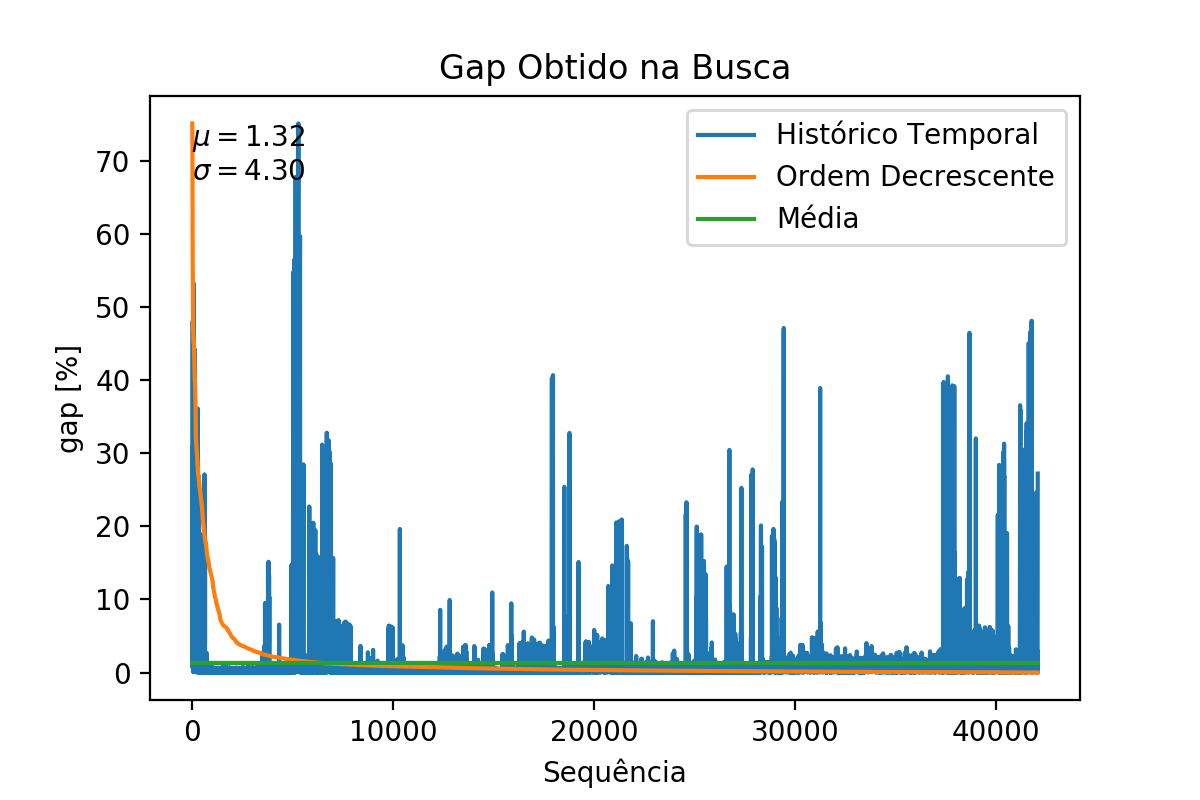
\includegraphics[width=1.0\linewidth]{figuras/hist}
	\caption[Teste 12 \--- Hist{\'o}rico de $gap$]{Teste 12 \--- Hist{\'o}rico de Gap [Fonte: Simula{\c c}{\~a}o]}
	\label{fig:Teste_12.hist}
\end{figure}

Portanto, a partir da visualiza{\c c}{\~a}o, torna-se evidente a discrep{\^a}ncia entre os valores que encontram-se acima e abaixo da m{\'e}dia. Ocorre que os valores que est{\~a}o abaixo da m{\'e}dia apresentam baixos valores de $gap$, pois j{\'a} encontram-se acomodados em torno de uma solu{\c c}{\~a}o {\'o}tima local, e apresentam apenas pequenos ajustes de acordo com a varia{\c c}{\~a}o nas cargas da rede. J{\'a} os valores mais altos ocorrem quando uma nova solu{\c c}{\~a}o inicial {\'e} gerada (quando h{\'a} mudan{\c c}a na topologia da rede ocasionada por entrada ou sa{\'\i}da de carga ou painel), tornando necess{\'a}ria a busca de um ponto otimizado a partir da nova solu{\c c}{\~a}o. Portanto, esses valores, classificados como $gap$ ``em acomoda{\c c}{\~a}o'', s{\~a}o os valores que ilustram o quanto a solu{\c c}{\~a}o otimizada se distancia da solu{\c c}{\~a}o inicial.

A Figura~\ref{fig:Teste_12.trans} apresenta os valores de $gap$ em ordem decrescente apenas dos valores acima da m{\'e}dia, classificados como regime em acomoda{\c c}{\~a}o. A m{\'e}dia destes valores, chamada de $gap_{medio}$, ser{\'a} utilizada para compara{\c c}{\~a}o entre os resultados para inferir a influ{\^e}ncia dos par{\^a}metros de ajuste sobre o comportamento do esquema apresentado.


\begin{figure}[!h]
	\centering
	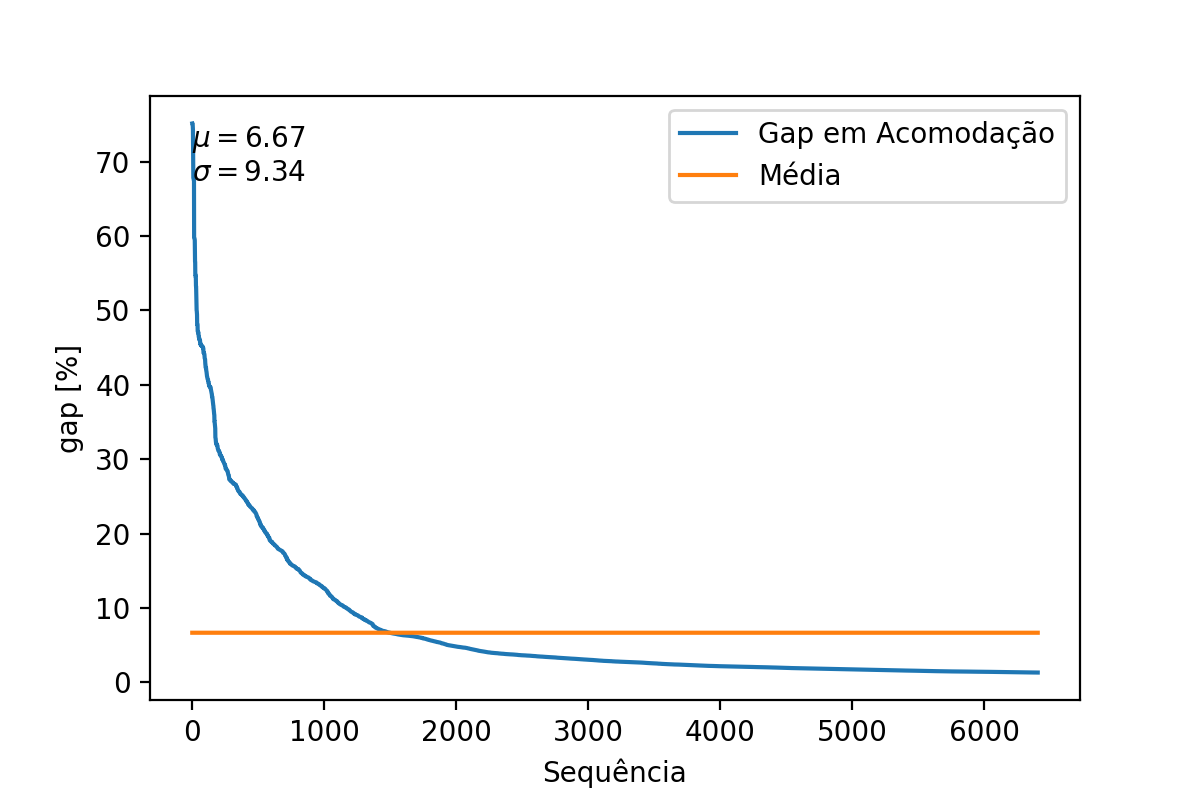
\includegraphics[width=1.0\linewidth]{figuras/trans}
	\caption[Teste 12 \--- Gap em Acomoda{\c c}{\~a}o]{Teste 12 \--- Gap em Acomoda{\c c}{\~a}o [Fonte: Simula{\c c}{\~a}o]}
	\label{fig:Teste_12.trans}
\end{figure}

A Tabela~\ref{tab:compara} apresenta os resultados obtidos nos 25 cen{\'a}rios de teste realizados.


\begin{table}[!h]
	\begin{center}
		\caption[Resumo dos Resultados \--- Par{\^a}metros Utilizados e M{\'e}dia de Ganhos no Regime de Acomoda{\c c}{\~a}o]{Resumo dos Resultados \--- Par{\^a}metros Utilizados e M{\'e}dia de Ganhos no Regime de Acomoda{\c c}{\~a}o [Fonte: Simula{\c c}{\~a}o]}
		\label{tab:compara}
		\vspace{5pt}
		\begin{tabular}{c c c c c c}
			\hline
			\textbf{Cen{\'a}rio de Teste} & \textbf{$C_{1}$} & \textbf{$C_{2}$} & \textbf{$C_{3}$} & \textbf{$C_{4}$} & \textbf{$gap_{medio}$} \\
			\hline\hline
			Teste 01 & 0 & 0 & 0 & 99 & 0.00 \\
			Teste 02 & 0 & 0 & 25 & 99 & 18.99 \\
			Teste 03 & 0 & 0 & 50 & 99 & 12.02 \\
			Teste 04 & 0 & 0 & 99 & 25 & 8.02 \\
			Teste 05 & 0 & 0 & 99 & 50 & 17.35 \\
			Teste 06 & 0 & 25 & 0 & 99 & 32.39 \\
			Teste 07 & 0 & 25 & 25 & 99 & 9.96 \\
			Teste 08 & 0 & 25 & 99 & 0 & 10.05 \\
			Teste 09 & 0 & 25 & 99 & 25 & 13.16 \\
			Teste 10 & 0 & 99 & 0 & 25 & 21.98 \\
			Teste 11 & 0 & 99 & 0 & 50 & 31.59 \\
			Teste 12 & 0 & 99 & 25 & 0 & 6.67 \\
			Teste 13 & 0 & 99 & 25 & 25 & 13.31 \\
			Teste 14 & 25 & 0 & 0 & 99 & 19.99 \\
			Teste 15 & 25 & 0 & 25 & 99 & 24.75 \\
			Teste 16 & 25 & 0 & 99 & 0 & 6.83 \\
			Teste 17 & 25 & 0 & 99 & 25 & 12.16 \\
			Teste 18 & 25 & 99 & 0 & 0 & 5.61 \\
			Teste 19 & 25 & 99 & 0 & 25 & 9.93 \\
			Teste 20 & 99 & 0 & 0 & 25 & 7.26 \\
			Teste 21 & 99 & 0 & 0 & 50 & 8.98 \\
			Teste 22 & 99 & 0 & 25 & 0 & 11.07 \\
			Teste 23 & 99 & 0 & 25 & 25 & 9.19 \\
			Teste 24 & 99 & 25 & 0 & 0 & 13.60 \\
			Teste 25 & 99 & 25 & 0 & 25 & 15.16 \\
			\hline
		\end{tabular}
	\end{center}
\end{table}

\section{An{\'a}lise dos Resultados} \label{sec:anares}

Observando o sum{\'a}rio de testes apresentado na Tabela~\ref{tab:compara}, observa-se que os dois primeiros fatores da Equa{\c c}{\~a}o~\ref{eq:obj}, quando ressaltados, trazem ganhos mais expressivos na busca, resultando em maiores altera{\c c}{\~o}es. Este comportamento {\'e} esperado, uma vez que s{\~a}o estes termos que diferem da solu{\c c}{\~a}o cl{\'a}ssica, expressa nos dois {\'u}ltimos termos. Ou seja, ao ressaltar a quantidade m{\'i}nima de cargas e a menor diferen{\c c}a de pot{\^e}ncia el{\'e}trica poss{\'\i}vel entre a carga efetivamente descartada e a carga que deve ser descartada, o sistema vai, na maioria das vezes, adequar a solu{\c c}{\~a}o predefinida para atender a estes requisitos. Assim, ganhos maiores na busca apenas ressaltam o quanto a solu{\c c}{\~a}o foi alterada sem interfer{\^e}ncia do operador, n{\~a}o fazendo, portanto, ju{\'\i}zo de valor sobre as cargas efetivamente selecionadas. Em outras palavras, n{\~a}o {\'e} um ganho absoluto, mas relativo {\`a} solu{\c c}{\~a}o anterior, que, por sua vez, pode j{\'a} ser suficientemente boa para n{\~a}o demandar muitas altera{\c c}{\~o}es.

Os testes realizados podem ser considerados satisfat{\'o}rios, pois demonstraram a versatilidade do m{\'e}todo proposto dentro dos cen{\'a}rios simulados, bem como uma tend{\^e}ncia de comportamento relativa a parametriza{\c c}{\~a}o dos ajustes.

H{\'a} uma parte da ferramenta que n{\~a}o foi explicitamente implementada na simula{\c c}{\~a}o. Por{\'e}m, os resultados obtidos corroboram sua efetividade. Trata-se da multiplicidade de crit{\'e}rios de opera{\c c}{\~a}o expressa na Equa{\c c}{\~a}o~\ref{eq:f3} que foi definida na Subsess{\~a}o~\ref{subsec:f3}. Para esta simula{\c c}{\~a}o, apenas um conjunto de crit{\'e}rios de import{\^a}ncia foi implementado, representando em si o resultado da m{\'e}dia ponderada entre os m{\'u}ltiplos cen{\'a}rios poss{\'\i}veis, ajustado para refletir a tabela est{\'a}tica da solu{\c c}{\~a}o cl{\'a}ssica. Entretanto, diversos conjuntos poderiam ser utilizados, e o valor final poderia ser uma sele{\c c}{\~a}o entre estes ou, ainda, uma combina{\c c}{\~a}o ponderada destes. 

O cen{\'a}rio Teste~01 que na meta-heur{\'\i}stica obteve $gap_{medio}$ nulo, demonstra um enorme poder de sucesso na sele{\c c}{\~a}o de m{\'u}ltiplos cen{\'a}rios. Assim, pode-se obter uma tabela est{\'a}tica (ou diretriz de solu{\c c}{\~a}o inicial) para o cen{\'a}rio de interesse, que, no caso de uma plataforma de petr{\'o}leo, poderia priorizar, por exemplo, os sistemas de produ{\c c}{\~a}o, facilidades ou seguran{\c c}a.

\chapter{Conclus{\~o}es e Trabalhos Futuros} \label{cap:concl}

Este trabalho construiu um sistema inteligente para tomada de decis{\~o}es na determina{\c c}{\~a}o de cargas a serem desligadas automaticamente, atrav{\'e}s de uma solu{\c c}{\~a}o de baixo impacto na rede, aplicando t{\'e}cnicas de intelig{\^e}ncia artificial a m{\'e}todos de atua{\c c}{\~a}o de rel{\'e}s.

Os testes realizados corroboraram a efic{\'a}cia do m{\'e}todo proposto, ainda que no campo da simula{\c c}{\~a}o, j{\'a} que testes em sistemas reais demandam um custo demasiado elevado, tornando-os invi{\'a}veis. Neste aspecto, o \textit{software} desenvolvido mostrou-se eficiente e robusto, pois, al{\'e}m de realizar uma simula{\c c}{\~a}o bastante completa do ponto de vista da din{\^a}mica do sistema de pot{\^e}ncia, tamb{\'e}m conseguiu simular os efeitos de prote{\c c}{\~a}o e atua{\c c}{\~a}o do sistema de rejei{\c c}{\~a}o autom{\'a}tica de cargas, bem como a fun{\c c}{\~a}o de busca, utilizando, para tanto, um hardware comum e acess{\'\i}vel.

Com a simula{\c c}{\~a}o realizada, foi utilizado o algoritmo de busca \textbf{VND} para fazer convergir a solu{\c c}{\~a}o para o menor custo encontrado, utilizando, para avalia{\c c}{\~a}o deste custo, a equa{\c c}{\~a}o proposta neste trabalho, que oferece ao operador a flexibilidade de definir par{\^a}metros do algoritmo para fugir da solu{\c c}{\~a}o cl{\'a}ssica, visando uma melhor adequa{\c c}{\~a}o aos requisitos el{\'e}tricos da rede.

Conforme descrito ao longo do trabalho, as solu{\c c}{\~o}es existentes s{\~a}o bastante detalhadas e consolidadas para atender ao problema do ponto de vista el{\'e}trico, e, eventualmente, econ{\^o}mico, no caso das concession{\'a}rias de distribui{\c c}{\~a}o. Entretanto, este trabalho visa combinar aspectos distintos para fornecer uma solu{\c c}{\~a}o diferenciada com m{\'u}ltiplos objetivos, aliando aspectos el{\'e}tricos e operacionais, permitindo ao operador definir o quanto a decis{\~a}o deve pender para um aspecto ou outro atrav{\'e}s dos par{\^a}metros de configura{\c c}{\~a}o.

Este trabalho foi, portanto, bem sucedido na proposta de aumentar a variedade de solu{\c c}{\~o}es dispon{\'\i}veis, agregando em si aspectos ben{\'e}ficos encontrados separadamente em outras solu{\c c}{\~o}es, sem perder a robustez computacional.

Trabalhos futuros s{\~a}o divisados, considerando que o escopo deste trabalho foi espec{\'\i}fico ao simular opera{\c c}{\~a}o de sistemas ilhados, embora o m{\'e}todo sugerido possa ser utilizado em sistemas conectados {\`a} rede el{\'e}trica p{\'u}blica, eletricamente chamada de barra infinita. Para tanto, a alimenta{\c c}{\~a}o da rede deve ser considerada como um gerador extra, cuja pot{\^e}ncia nominal seja a pot{\^e}ncia para qual a prote{\c c}{\~a}o da entrada atue por sobrecorrente. Esse t{\'o}pico configura um estudo em aberto.

Outra limita{\c c}{\~a}o considerada aqui {\'e} a gera{\c c}{\~a}o concentrada na subesta{\c c}{\~a}o principal. Este normalmente {\'e} o caso de sistemas ilhados, como plataformas de petr{\'o}leo, plantas industriais de produ{\c c}{\~a}o ou estabelecimentos comerciais que operem offline em hor{\'a}rio de ponta. Entretanto, redes que alimentem sistemas de trem ou metr{\^o}, por exemplo, podem ter a gera{\c c}{\~a}o distribu{\'\i}da por subesta{\c c}{\~a}oes diversas. A simula{\c c}{\~a}o de tais casos demanda um esfor{\c c}o significativo na constru{\c c}{\~a}o de um sistema de simula{\c c}{\~a}o, e, traz como benef{\'\i}cio a possibilidade de aplicar esta filosofia em redes de grande porte, tanto de distribui{\c c}{\~a}o quanto de transmiss{\~a}o. Assim, tais sistemas fornecem um complexo e desafiador problema a ser estudado.

Este trabalho abriu uma possibilidade ampla de considerar como as rela{\c c}{\~o}es entre cargas n{\~a}o conectadas eletricamente se influenciam mutuamente. Este, talvez seja um dos aspectos mais importantes acrescentados aqui. Entretanto, pela dificuldade de simula{\c c}{\~a}o desses fen{\^o}menos que surgem na aplica{\c c}{\~a}o pr{\'a}tica, este aspecto n{\~a}o foi devidamente explorado. Trata-se da matriz de correla{\c c}{\~a}o que entra na Equa{\c c}{\~a}o~\ref{eq:f0} e foi citada na Se{\c c}{\~a}o~\ref{subsec:f1} como sendo a matriz de topologia da rede. A simula{\c c}{\~a}o realizada aqui considerou a topologia da rede como {\'u}nica rela{\c c}{\~a}o entre as cargas, ou seja, a conex{\~a}o el{\'e}trica entre estas. Todavia, as conex{\~o}es mec{\^a}nicas ou outras conex{\~o}es f{\'\i}sicas tamb{\'e}m podem fazer com que duas cargas distintas se influenciem. Por exemplo, uma bomba \textit{booster}, que {\'e} utilizada para elevar a press{\~a}o de um fluido antes que este chegue {\`a} suc{\c c}{\~a}o de uma bomba principal, representa uma conex{\c c}{\~a}o puramente mec{\^a}nica, j{\'a} que estas operam, geralmente, em circuitos el{\'e}tricos distintos. Entretanto, em situa{\c c}{\~o}es espec{\'\i}ficas de desligamento inesperado, o sa{\'\i}da da primeira causa baixa press{\~a}o no fluido que chega {\`a} segunda, fazendo com que a mesma tamb{\'e}m desligue inesperadamente. Este importante aspecto pode ser considerado no modelo ao substituir o elemento da linha correspondente {\`a} carga desligada e coluna correspondente {\`a} carga influenciada pelo valor \textit{True}. Assim, uma sugest{\~a}o para continua{\c c}{\~a}o deste trabalho {\'e} a elabora{\c c}{\~a}o de um m{\'o}dulo que opera junto ao supervis{\'o}rio de opera{\c c}{\~a}o do sistema, monitorando o comportamento em tempo real objetivando manter esta matriz atualizada. Assim, o projetista do sistema, ao considerar sua experi{\^e}ncia em conjunto com os operadores, pode inserir uma estimativa inicial para os casos que podem ser previstos enquanto um software se encarrega de atualizar o restante durante a opera{\c c}{\~a}o. Por exemplo, cada vez que uma carga {\'e} desligada, o sistema monitora os segundos seguintes e insere incrementos para cada carga adicional desligada, com valor inversamente proporcional ao tempo decorrido, e decrementos para valores altos sem desligamento concretizado. Para um valor de fronteira definido, o elemento correspondente na matriz de correla{\c c}{\~a}o torna-se \textit{True}. Tal metodologia figura apenas como sugest{\~a}o, devendo seus aspectos e comportamentos serem analisados {\`a} parte.